\documentclass[UTF8,zihao=-4,a4paper,fontset=fandol]{ctexart}
\usepackage{cumcm-paper}

\setlength{\tabcolsep}{5pt}
\renewcommand{\arraystretch}{1.18}

\title{“拍照赚钱”的任务定价}
\author{}
\date{}

\begin{document}

\maketitle

\begin{cumcmabstract}
\hspace{2em}本文针对移动众包平台“拍照赚钱”任务的定价与发布问题，基于历史任务、会员位置和新任务数据，构建“空间供需诊断--完成概率估计--单任务定价--任务包优化”的统一框架。结果均为基于历史数据的模型预测，重点回答四问所要求的定价规律、改进价格、打包效果和新任务实施方案。

\hspace{2em}针对问题一，本文构造价格、最近会员距离、2 km 邻域供需和相对价格等指标，建立带城市固定效应的 Logistic 模型。835个任务中522个完成，完成率为62.51\%；任务模型加入城市效应后AUC由0.700提高到0.829。深圳161个任务实际完成率仅21.74\%，而任务变量模型期望为48.95\%，存在$-27.21$个百分点残差。由此判断原方案虽有“会员密集区低价、偏远区补偿”的规律，却未充分计入区域综合执行条件；交通拥堵只能作为背景佐证，不能据四城市数据作因果结论。\aimark{1}

\hspace{2em}针对问题二，本文以带 $L_2$ 正则和价格单调约束的 Logistic 模型计算0.5元步长候选价格的完成概率，再建立含预算、$\pm8$元调价幅度、价格稳定性和区域服务下限的多选择背包MILP。推荐方案把平均价格由69.11元调为73.61元，预计支付由36444.28元增至41910.85元，预测完成数由522.00个增至573.96个，预测完成率由62.52\%增至68.74\%。\aimark{2}

\hspace{2em}针对问题三，本文筛选单任务优化后概率仍低于0.5且达到调价边界的任务作为核心，以1 km邻域和最小生成树路线构造2--5任务的紧凑任务包，并联合选择单任务价格和包价格。同问题二预算下选取46个任务包、覆盖120个任务，预测完成数达到584.55个、完成率达到70.01\%，比问题二增加10.60个预计完成任务；预算放宽1\%和2\%时完成率分别为70.38\%和70.75\%。\aimark{3}

\hspace{2em}针对问题四，本文对附件三2066个新任务重新计算有效会员供给与任务压力，生成自适应紧凑任务包，并以会员预订限额约束包的指派。优化方案选择971个发布单元，其中709个为多任务包、覆盖1804个任务，分配391名会员且无人超限；平均单价84.11元，预计支付111842.52元，预测完成1332.11个，预测完成率64.48\%。该结果是容量约束下的新任务发布建议，应以小规模试运行校准。\aimark{4}
\end{cumcmabstract}

\keywords{众包任务定价；空间供需；任务打包；Logistic回归；混合整数规划}

\CumcmBodyStart

\section{问题重述}

“拍照赚钱”平台将商业检查任务发布给注册会员，会员根据位置、时间与报酬选择任务并上传照片。若标价不足以补偿会员的出行和执行成本，任务可能无人领取；若平台一味提高标价，又会扩大支付支出。因此，合理定价需要同时处理任务吸引力、局部供需和平台成本三者之间的关系。

附件一给出835个已结束任务的位置、标价和完成状态，附件二给出1877名会员的位置、预订限额、开始预订时间及信誉值，附件三给出2066个新任务的位置。问题一要求识别历史定价规律和未完成原因；问题二要求重新定价；问题三要求研究集中任务的打包发布；问题四要求为新任务制定价格。四问形成“解释历史--优化单价--联合打包--迁移实施”的递进关系。

\section{问题分析}

问题一的难点在于，价格和完成状态都具有空间异质性。若只比较不同价格组的平均完成率，容易把区域差异、会员密度和任务竞争混入价格效应；若只观察会员数量，又会忽略注册会员并不等于有效会员。因此，本文建立地理距离和局部邻域，从低价、有效供给、区域效应和任务竞争四条证据链解释未完成现象。

问题二不能采用统一加价。不同任务的价格敏感程度并不相同：有些任务少量加价即可提高完成概率，有些任务即使大幅加价仍受区域困难限制；同时，高完成概率区域存在适度降价空间。为此，本文先估计每个任务的价格--完成概率响应，再在离散候选价格中选择一项，使预计完成任务数尽可能大。主成本口径采用“价格乘预测完成概率”的预计支付金额，全部标价总额只作为补充指标。

问题三判断相邻任务能否通过联合发布把竞争关系转化为路线协同。若任务距离较近，会员一次出行可以完成多个检查点，包内总报酬提高、单位绕行成本下降；但包过大或路线过长又会降低整包接受概率。因此，本问由问题二识别低概率核心困难任务，再构造紧凑候选包，并让单任务发布和打包发布在同一预算约束下竞争。

问题四面对附件三的新任务，不能只照搬历史任务的重新定价结果。新任务数量、空间密集程度和有效会员供给都可能偏离历史样本，直接套用前三问价格和打包概率会高估高密度区域完成能力。因此，本问把价格响应、任务包构造和区域压力指标迁移到新任务，同时加入会员预订限额约束，给出容量约束发布方案。

四问的信息流为：历史任务与会员数据形成空间特征；原标价和空间特征解释完成状态；完成概率模型给出候选价格的成功概率；单任务优化模型输出新价格；打包模型处理困难任务；新任务模型根据附件三分布和会员容量完成迁移定价，并以基线比较、预算敏感性、覆盖唯一性和分布迁移检查评价方案。

\subsection{总体建模框架}

从决策对象看，任务位置和会员分布属于给定环境，任务价格和发布方式属于平台可控变量，任务是否完成属于随机结果。问题一解释原方案失效原因；问题二转为单任务价格决策；问题三新增任务包选择变量；问题四把历史模型迁移到新任务并增加会员容量约束。因此，四问虽共享同一完成概率口径，但依次对应解释、单价优化、联合发布和新任务实施。

在空间层面，本文用三个尺度刻画任务环境。点尺度使用任务价格和最近会员距离；邻域尺度使用2 km内会员数量、会员能力、任务数量和相对价格；区域尺度用空间聚类虚拟变量吸收更广范围的综合差异。这种分层避免用单一会员密度解释所有现象。

在统计层面，先用分组完成率和静态地图描述事实，再用模型控制多个因素。描述性统计用于发现稳定模式；Logistic模型把位置和会员环境转化为候选价格下的可比概率；MILP不重新估计概率，只在给定概率和成本矩阵上选择价格。由此，数据分析、概率估计与价格优化的职责相互分离。

\section{模型假设}

为使模型能够由现有附件求解，作如下必要假设。

\begin{enumerate}[label=\arabic*)]
  \item 在同一批任务的重新定价比较中，任务位置、任务内容和会员总体分布保持不变，价格是可控变量；未观测到的交通和商业环境由区域变量近似吸收。
  \item 会员通常优先考虑距离较近、报酬较高且可在预订限额内完成的任务，因此距离衰减、会员能力和邻近任务竞争可以用于刻画任务吸引力。
  \item 其他条件相同时，提高任务价格不会降低其完成概率，故在完成概率模型中对价格系数施加非负约束。
  \item 平台仅对完成任务支付标价，因此新方案的成本以预计支付金额度量；未完成任务产生的管理成本因附件缺少数据而不计。
\end{enumerate}

\section{符号说明}

\begin{table}[H]
  \centering
  \caption{本文主要符号及其含义}
  \label{tab:symbols}
  \begin{tabular}{clc}
    \toprule
    符号 & 含义 & 单位 \\
    \midrule
    $P_i$ & 任务 $i$ 的原标价 & 元 \\
    $P_{ik}$ & 任务 $i$ 的第 $k$ 个候选价格 & 元 \\
    $Y_i$ & 任务完成状态，完成为1，否则为0 & -- \\
    $d_{ij}$ & 任务 $i$ 与会员 $j$ 的球面距离 & km \\
    $D_i$ & 任务 $i$ 到最近会员的距离 & km \\
    $N_i$ & 任务 $i$ 周围2 km内会员数量 & 人 \\
    $G_i$ & 任务 $i$ 周围2 km内其他任务数量 & 个 \\
    $Q_i,H_i$ & 周围会员预订限额之和、信誉值之和 & -- \\
    $K_i$ & 任务 $i$ 的局部竞争强度 & -- \\
    $p_i(P)$ & 任务 $i$ 在价格 $P$ 下的预测完成概率 & -- \\
    $x_{ik}$ & 是否为任务 $i$ 选择候选价格 $P_{ik}$ & -- \\
    $C_0,C_{\max}$ & 原方案预计支付金额及成本上限 & 元 \\
    \bottomrule
  \end{tabular}
\end{table}

\section{数据预处理与空间指标}

\subsection{数据清洗与描述}

附件一包含835条历史任务记录，其中完成任务522个、未完成任务313个，历史实际完成率为62.51\%。任务价格在65--85元之间，平均价格为69.11元，中位数为67元。附件二包含1877名会员。本文统一将经纬度转为数值型，检查任务编号和位置字段，对会员位置字符串拆分为纬度、经度，并保留预订限额、信誉值和开始预订时间等能力信息。

完成任务的平均价格为69.82元，未完成任务的平均价格为67.93元，二者相差1.89元。这个差异提示价格与完成状态相关，但不能直接解释为因果关系，因为平台可能已经对偏远任务进行了加价。后续模型因此同时控制空间供需和区域变量。

\subsubsection{坐标与状态一致性处理}

任务和会员坐标均位于珠三角相邻经纬度范围内，先检查纬度、经度是否落入研究区的合理边界，再以任务编号作为逐任务结果表的唯一索引。执行状态统一转换为二元变量，价格保留0.5元精度。由于空间距离直接进入邻域计数和最近距离，如果经纬度顺序颠倒会造成数百千米误差，因此在计算前分别检查纬度约为22--24度、经度约为113--115度，并用广州、东莞、深圳三个明显点群进行地图复核。

对于会员数据，位置字段以“纬度 经度”形式存储，拆分后与任务坐标采用同一坐标次序。预订限额和信誉值既反映会员能承担多少任务，也可能与会员优先预订时间相关。本文不把三者机械相加，而是在概率模型中分别统计邻域累计限额和累计信誉，使模型能够从历史完成状态中估计它们在给定价格下的净关联。

\subsubsection{尺度选择与数值变换}

邻域半径过小会导致大量任务周围会员数为零，指标离散且不稳定；半径过大则会把跨城区、跨江或通勤上不可达的会员视为同一供给。结合珠三角城市任务密度，本文以2 km作为主要局部尺度，同时在前期检查1 km和5 km统计。2 km尺度既能形成足够的邻居数量，又能保留广州中心、东莞和深圳之间的明显差异。

会员数量、邻近任务数量、限额和信誉累计值均呈右偏分布。若直接进入线性预测子，少数高密度点会主导系数。因此，对这些变量使用 $\ln(1+x)$ 变换；连续变量在拟合前进一步减去均值并除以标准差。标准化使 $L_2$ 惩罚对不同量纲的变量具有可比作用，也便于把价格系数限制为非负。

\subsubsection{地图编码与统计口径}

地图采用同一研究范围和卫星底图，避免因视野变化造成视觉误判。价格按65--69.5元、70--74.5元、75--79.5元和80--85元分为四档；圆点表示完成，叉号表示未完成。周边会员数量按0--2人、3--5人、6--10人和11人及以上分组；局部竞争强度按样本四分位数分组；区域未完成率则在至少包含3个任务的六边形网格上计算，以避免单点决定颜色。

所有分组统计均以任务为观测单位。完成率是组内 $Y_i$ 的算术平均，平均价格是组内 $P_i$ 的算术平均。六边形颜色和分组完成率只用于描述空间关系，不直接进入优化目标；优化模型使用逐任务概率，从而避免先分组再定价造成的信息损失。

\subsection{地理距离与局部邻域}

设任务与会员的经纬度分别为 $(\varphi_i,\lambda_i)$ 和 $(\varphi_j,\lambda_j)$，采用 Haversine 公式计算球面距离：
\begin{equation}
d_{ij}=2R\arcsin\sqrt{
\sin^2\frac{\varphi_i-\varphi_j}{2}
+\cos\varphi_i\cos\varphi_j
\sin^2\frac{\lambda_i-\lambda_j}{2}},
\label{eq:haversine}
\end{equation}
其中地球平均半径 $R=6371$ km。由式\eqref{eq:haversine}得到最近会员距离
\begin{equation}
D_i=\min_j d_{ij},
\label{eq:nearest}
\end{equation}
并统计1 km、2 km和5 km邻域内的会员及任务数量。综合数据密度与城市出行尺度，正文以2 km邻域为主要分析口径。

简单会员数量无法反映会员能否实际执行任务。为表达距离、信誉和预订能力的共同作用，可定义有效供给
\begin{equation}
S_i=\sum_j I(d_{ij}\le r)\,w_j\exp(-\lambda d_{ij}),
\label{eq:supply}
\end{equation}
其中 $w_j$ 由会员信誉值、预订限额和开始预订时间综合确定。实际概率模型分别保留会员数量、限额之和与信誉值之和，以避免经验权重掩盖不同因素的作用。

\subsection{任务密度与局部竞争}

任务密度 $G_i$ 表示2 km内除任务 $i$ 外的其他任务数量。若邻近任务价格更高，当前任务面临的替代压力更大，因此定义局部竞争强度
\begin{equation}
K_i=\sum_{k\ne i}I(d_{ik}\le2)
\exp\left(\frac{P_k-P_i}{5}\right).
\label{eq:competition}
\end{equation}
式\eqref{eq:competition}同时考虑邻近任务数量和相对价格。当附近任务与本任务同价时，每个邻近任务贡献1；高出5元时贡献约为原来的 $e$ 倍。该指标用于问题一的原因分析，问题二的完成概率模型则以 $G_i$ 及区域虚拟变量吸收稳定的竞争环境。

\subsection{空间计算的实现}

严格距离由式\eqref{eq:haversine}定义。考虑到所有点都位于较小纬度范围，批量邻域搜索时将经度乘以 $111\cos\bar\varphi$、纬度乘以111，得到单位近似为km的局部平面坐标，再用KD树查询2 km内的会员和任务。该近似只用于加速邻居检索，不改变论文中的距离定义；对于研究区尺度，误差远小于2 km分组宽度。

对每个任务，先查询最近会员距离和邻域会员索引，再对索引对应的限额、信誉值求和。任务与任务之间使用另一棵KD树，并从邻居集合中排除任务自身。这样无需显式保存835乘1877的完整距离矩阵，计算量由逐对比较降为邻域查询，更适合在后续价格情景中重复使用固定空间特征。

最终特征表的一行对应一个任务，包含原价格、最近会员距离、会员数、任务数、会员限额之和、信誉值之和及区域编号。除价格外，这些特征在问题二的反事实定价中保持不变；每次改变候选价格时，只更新设计矩阵的价格列。该处理确保同一任务不同价格之间的概率差异只来自价格响应，而不是同时改变位置和供给环境。

\section{问题一：原任务定价规律及未完成原因}

\subsection{任务价格与完成状态的总体规律}

按价格划分后，低价任务占历史样本的主体。表\ref{tab:price-band}显示，65--69.5元共有510个任务，完成率仅54.1\%；当价格提高至70元以上时，完成率上升到74\%以上。价格从最低组到最高组增加约15元，完成率增加28.4个百分点，说明报酬是会员选择任务的重要因素。

\begin{table}[H]
  \centering
  \caption{不同价格区间的历史任务完成情况}
  \label{tab:price-band}
  \begin{tabular}{lrrr}
    \toprule
    价格区间/元 & 任务数/个 & 完成率/\% & 价格特征 \\
    \midrule
    65--69.5 & 510 & 54.1 & 样本最多、失败集中 \\
    70--74.5 & 207 & 74.4 & 完成率明显上升 \\
    75--79.5 & 78  & 75.6 & 边际提升趋缓 \\
    80--85   & 40  & 82.5 & 完成率最高 \\
    \bottomrule
  \end{tabular}
\end{table}

将任务点接入卫星地图后，图\ref{fig:q1-spatial}进一步显示：未完成任务不是均匀随机分布，而是在深圳以及广州、佛山部分任务密集区形成连续聚集；东莞附近则以完成任务为主。北部和外围任务虽然离城市中心较远，但多采用绿色、黄色或红色的较高价格，完成状态反而较好。这说明“距离远”不是失败的充分条件，关键在于价格是否补偿了局部执行成本。

\begin{figure}[H]
  \centering
  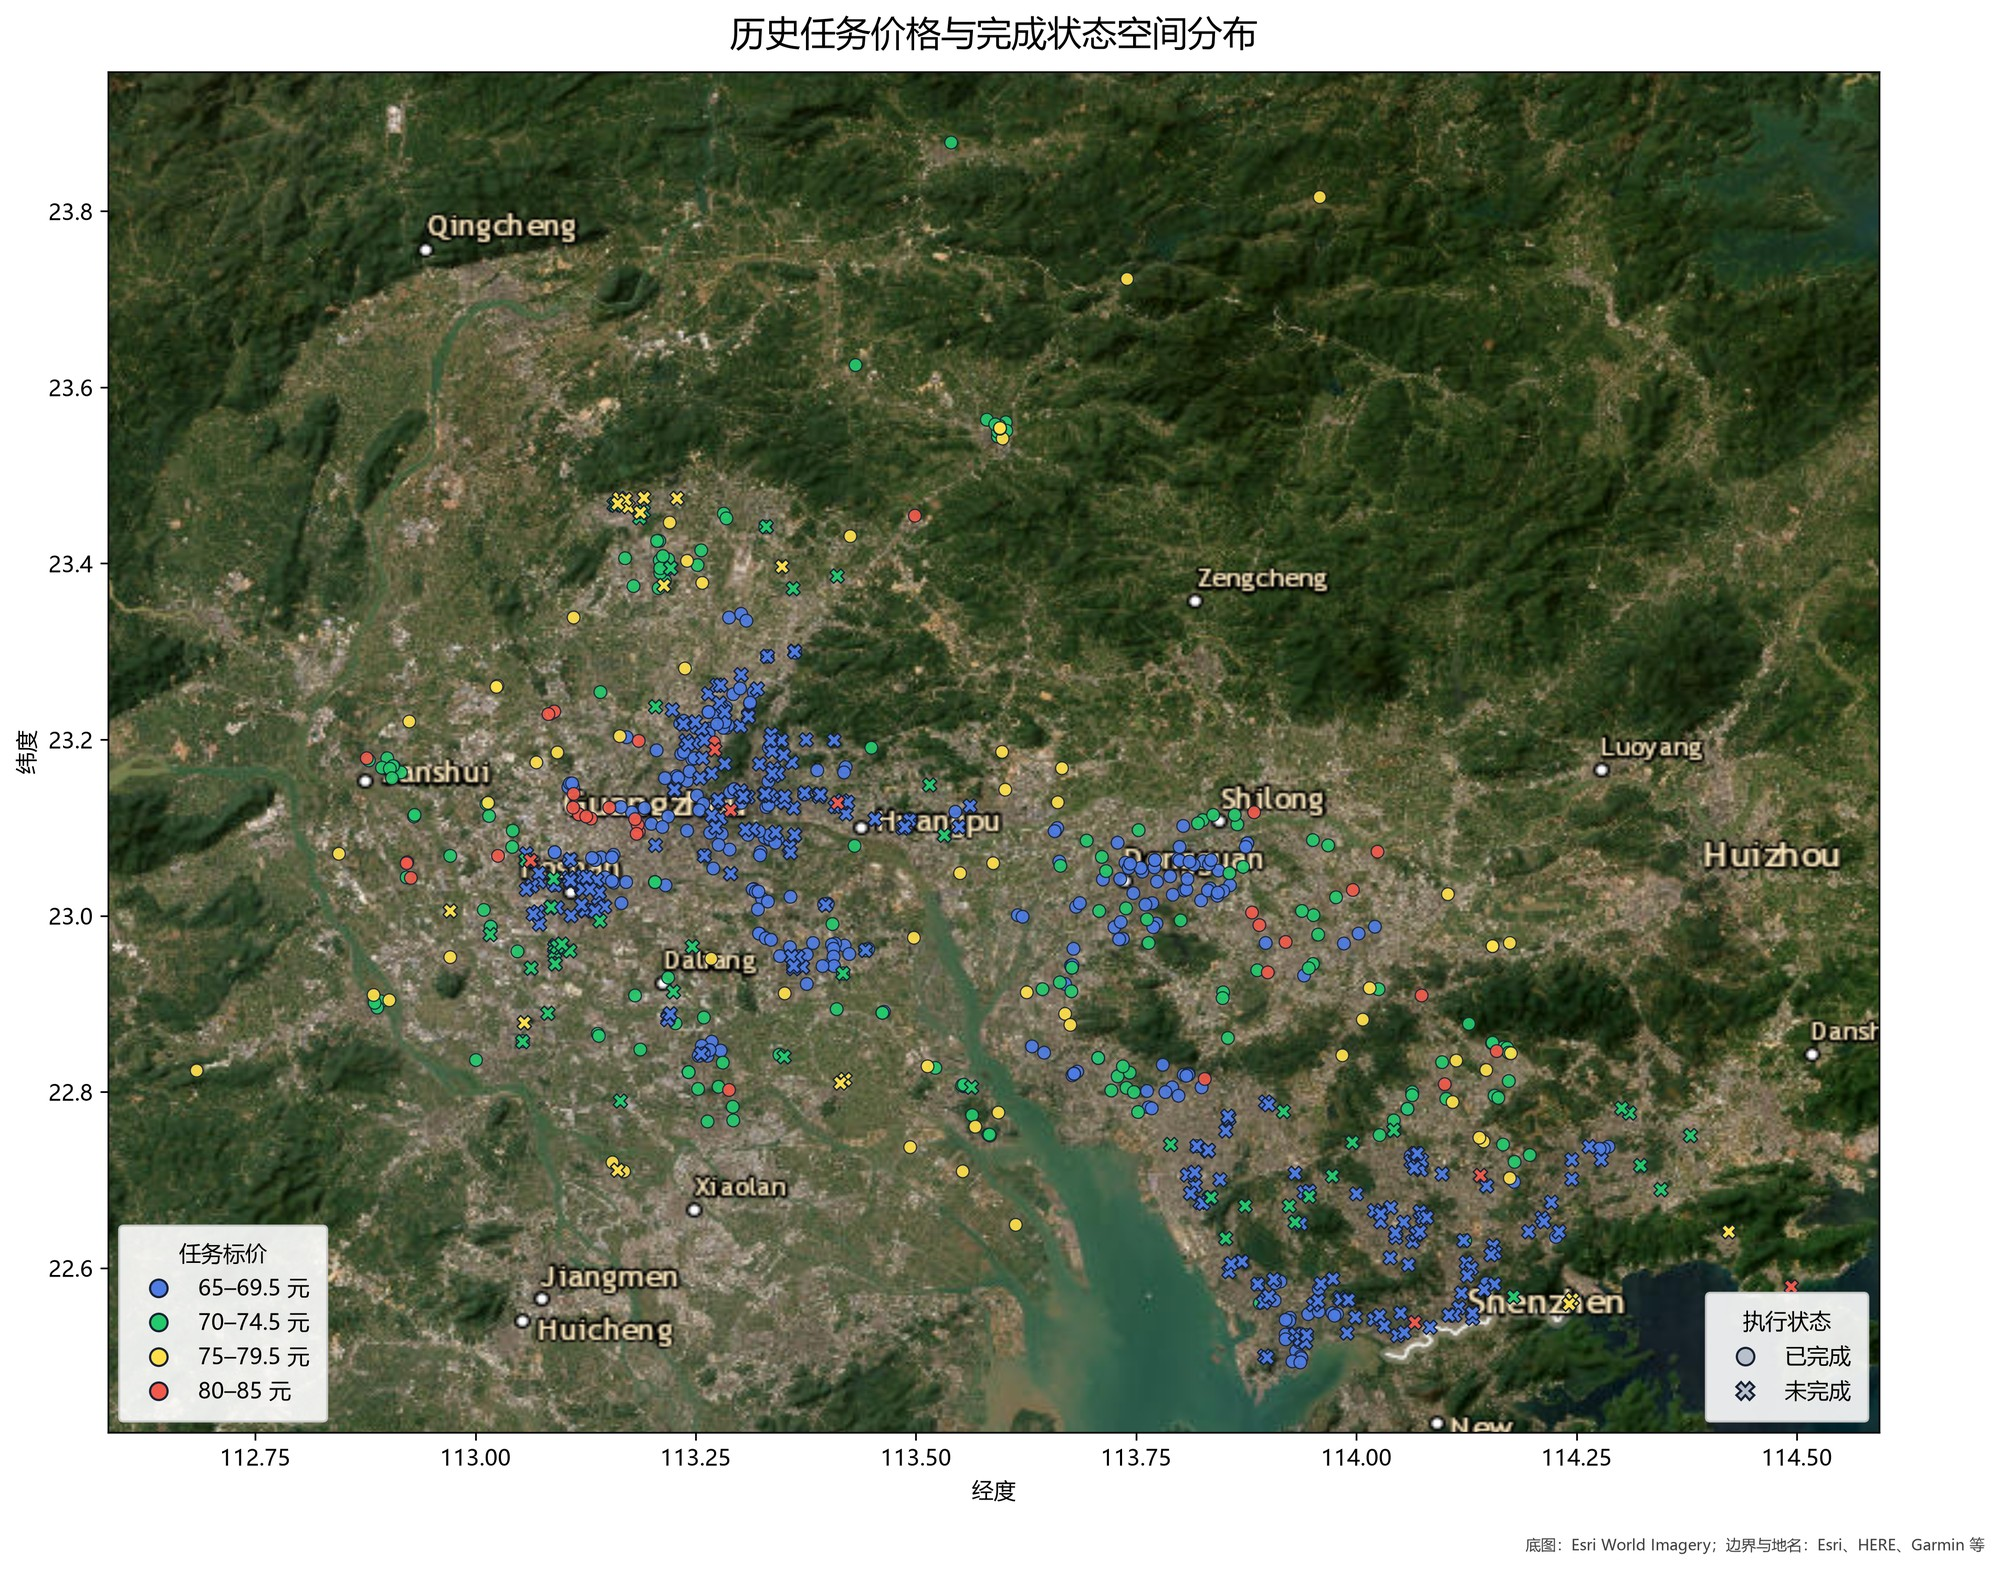
\includegraphics[width=0.96\textwidth]{../figures/fig-q1-spatial-v1.jpg}
  \caption{历史任务价格与完成状态的空间分布}
  \label{fig:q1-spatial}
\end{figure}

最低价格组包含61.1\%的历史任务，也是未完成任务的主要来源。价格提高到70元以上后，完成率跃升20个百分点以上，而继续提高至75--79.5元仅增加1.2个百分点，提示价格响应边际递减。最高价组只有40个样本，其82.5\%完成率不能直接外推。结合空间分布可知，失败取决于价格相对局部成本和替代任务的吸引力，而非距离或行政区域单独决定。

广州--佛山区域同时出现完成点与未完成点，说明同一大区域内部仍有任务级差异。中心城区任务与会员都较密集，但大量低价任务彼此相邻，会员会在多个候选任务之间选择；外围任务虽然距离较远，平台往往已提高价格进行补偿。东莞附近不少低价任务仍然完成，而深圳即使会员较多仍形成连续未完成带。这组对照说明区域变量只能吸收平均差异，最终失败取决于标价、局部供需和替代任务的共同作用。

\subsection{原任务定价规律}

为解释平台原标价，建立探索性价格模型
\begin{equation}
P_i=\beta_0+\beta_1D_i+\beta_2S_i+\beta_3G_i
+\sum_r\gamma_rR_{ir}+\varepsilon_i,
\label{eq:price-model}
\end{equation}
其中 $R_{ir}$ 为空间区域虚拟变量。仅使用最近会员距离、2 km内会员数、1 km内任务数等基础特征时，可解释约29\%的价格差异。估计结果的主要方向为：附近会员越多，原价格总体越低；任务位置越偏远，平台越倾向于给出补偿；任务聚集区的价格略低。

由此可概括原定价规则为“预期供给充足的区域降低标价，预期供给不足或位置偏远的区域提高标价”。这个原则本身具有合理性，但其供给代理变量过于依赖注册会员密度，没有充分扣除会员时间、限额、信誉和任务占用等限制，也没有区分任务聚集带来的顺路便利与任务之间的选择竞争。原模型的空间错配正是后续未完成任务聚集的来源。

约29\%的解释度表明，位置和简单供需指标进入了原定价逻辑，但任务类型、发布时间和平台内部规则等因素仍未被解释。因此本文不复原内部算法，只提取与重新定价有关的稳定方向：会员密度较高时原价倾向下降，而任务竞争可能抵消名义供给优势。问题二据此将完成概率写成价格、距离、供给、竞争和区域的函数，并只对价格作反事实变化。

会员密度与原价格的负向关系尤其值得注意。若平台把附近注册人数直接当作可执行供给，就会在广州、深圳等会员密集区持续给出低档价格；但这些会员同时覆盖大量任务，名义供给优势会被任务竞争抵消。相反，会员稀疏区域获得了距离补偿，反而可能保持较高完成率。这种“距离不利被价格补偿、密度有利被低价抵消”的交叉关系，也是简单相关分析出现反直觉方向的原因。

\subsection{原因一：低价不足以覆盖执行成本}

会员接受任务时更关注净收益而非名义标价。可将会员 $j$ 对任务 $i$ 的效用写为
\begin{equation}
U_{ij}=P_i-C_d(d_{ij})-C_t-C_h,
\label{eq:utility}
\end{equation}
其中 $C_d$ 为距离成本，$C_t$ 为时间成本，$C_h$ 为交通、停车或任务难度等综合成本。当可执行会员的 $U_{ij}$ 均低于接受阈值时，任务不会被完成。

结合表\ref{tab:price-band}与图\ref{fig:q1-spatial}，65--69.5元组的完成率比70--74.5元组低20.3个百分点，且低价未完成任务集中在深圳和广州部分密集区。这表明绝对收益不足与相邻高价任务的相对竞争共同作用。故问题二不对历史失败任务统一加价，而是拟合全部任务的完成概率，再比较同一任务不同候选价格的边际提升。

\subsection{原因二：注册会员数量高估了有效供给}

若注册会员数量能够代表真实供给，则会员密集区域应更容易完成任务；但表\ref{tab:supply-group}呈现相反的表面关系。2 km内会员不超过2人的任务完成率为79.4\%，而11人及以上组仅为42.9\%。与此同时，两组平均价格分别为71.89元和66.09元，说明平台很可能因附近注册会员较多而系统性压低价格。

\begin{table}[H]
  \centering
  \caption{周边会员数量分组的价格与完成率}
  \label{tab:supply-group}
  \begin{tabular}{lrrr}
    \toprule
    2 km内会员数 & 任务数/个 & 平均价格/元 & 完成率/\% \\
    \midrule
    0--2人 & 252 & 71.89 & 79.4 \\
    3--5人 & 210 & 70.00 & 68.6 \\
    6--10人 & 182 & 67.40 & 52.7 \\
    11人及以上 & 191 & 66.09 & 42.9 \\
    \bottomrule
  \end{tabular}
\end{table}

表中的负相关不能解释为“会员越多越不利”，而是注册数量、低价和任务竞争同时出现。注册会员还会受预订限额、信誉、任务占用和可接受距离折减；同一会员覆盖多个邻近任务时又会被重复计数。因此“11人及以上”不等于11名独立有效劳动力。问题二以会员限额、邻域任务数和区域变量近似有效供给。\aimark{3}

\begin{figure}[H]
  \centering
  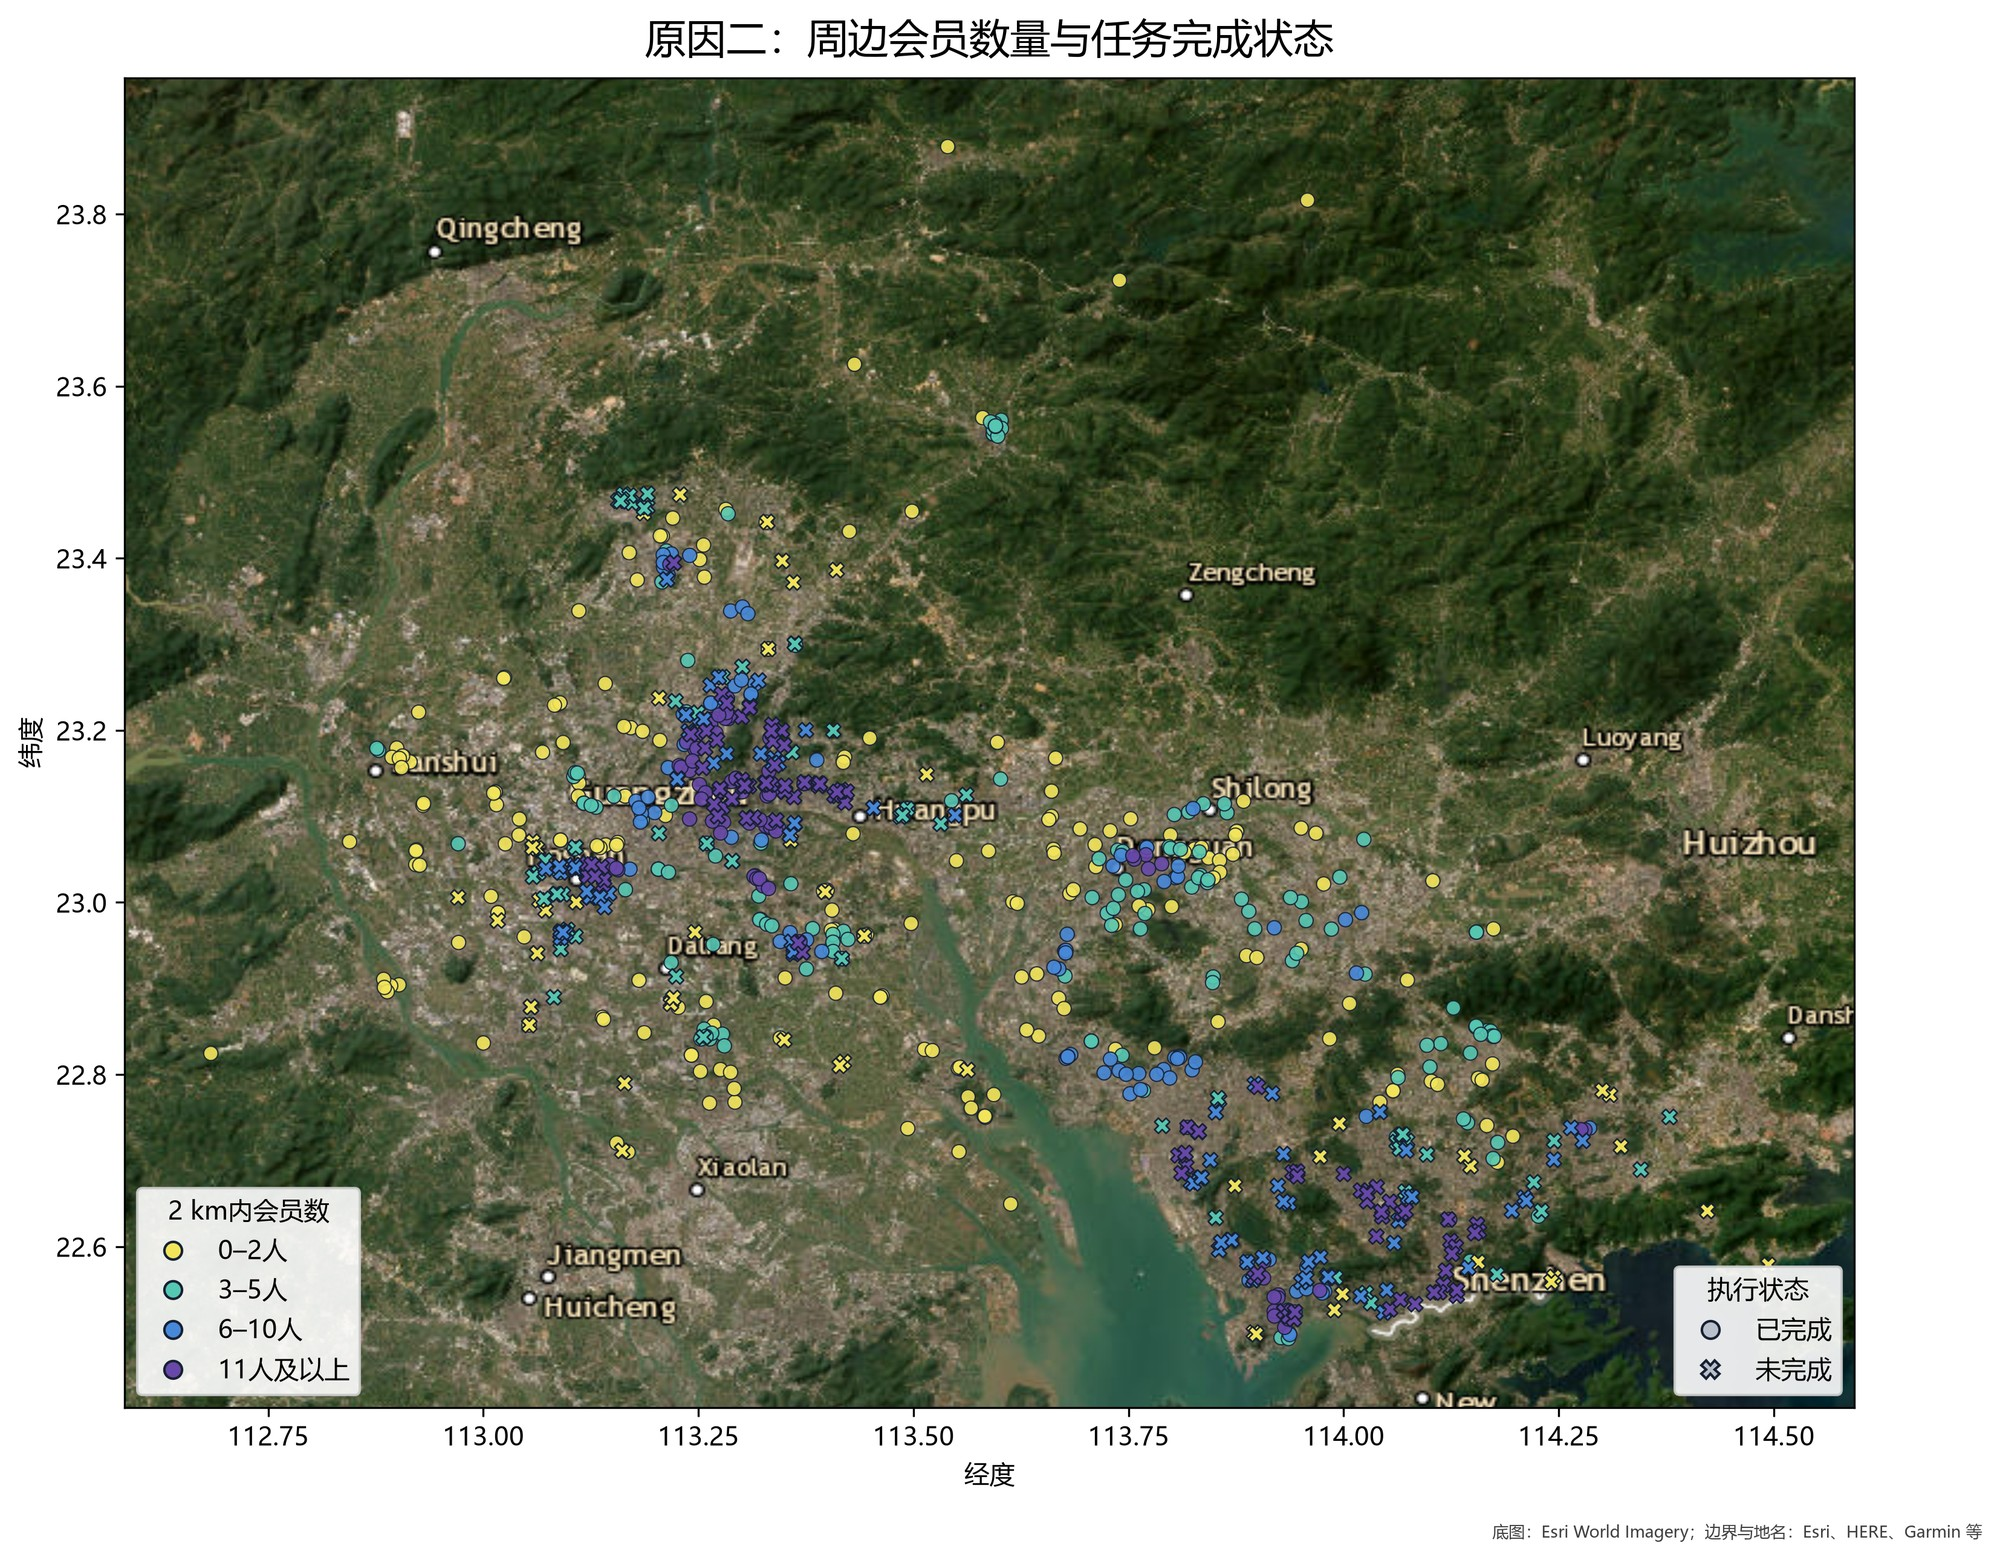
\includegraphics[width=0.96\textwidth]{../figures/fig-q1-supply-v1.jpg}
  \caption{周边会员数量与任务完成状态的空间分布}
  \label{fig:q1-supply}
\end{figure}

\subsection{原因三：区域综合执行成本未被充分补偿}

图\ref{fig:q1-region}按空间六边形统计局部未完成率，每个网格至少包含3个任务。深圳附近形成连续的高未完成率带，广州、佛山也存在若干高值网格，而东莞附近多为低值。探索性空间分组见表\ref{tab:q1-region}：深圳附近平均价格约68.30元、完成率约35.4\%；东莞附近平均价格约70.08元、完成率约97.0\%。两地平均价格只差约1.78元，完成率却相差61.6个百分点。

\begin{figure}[H]
  \centering
  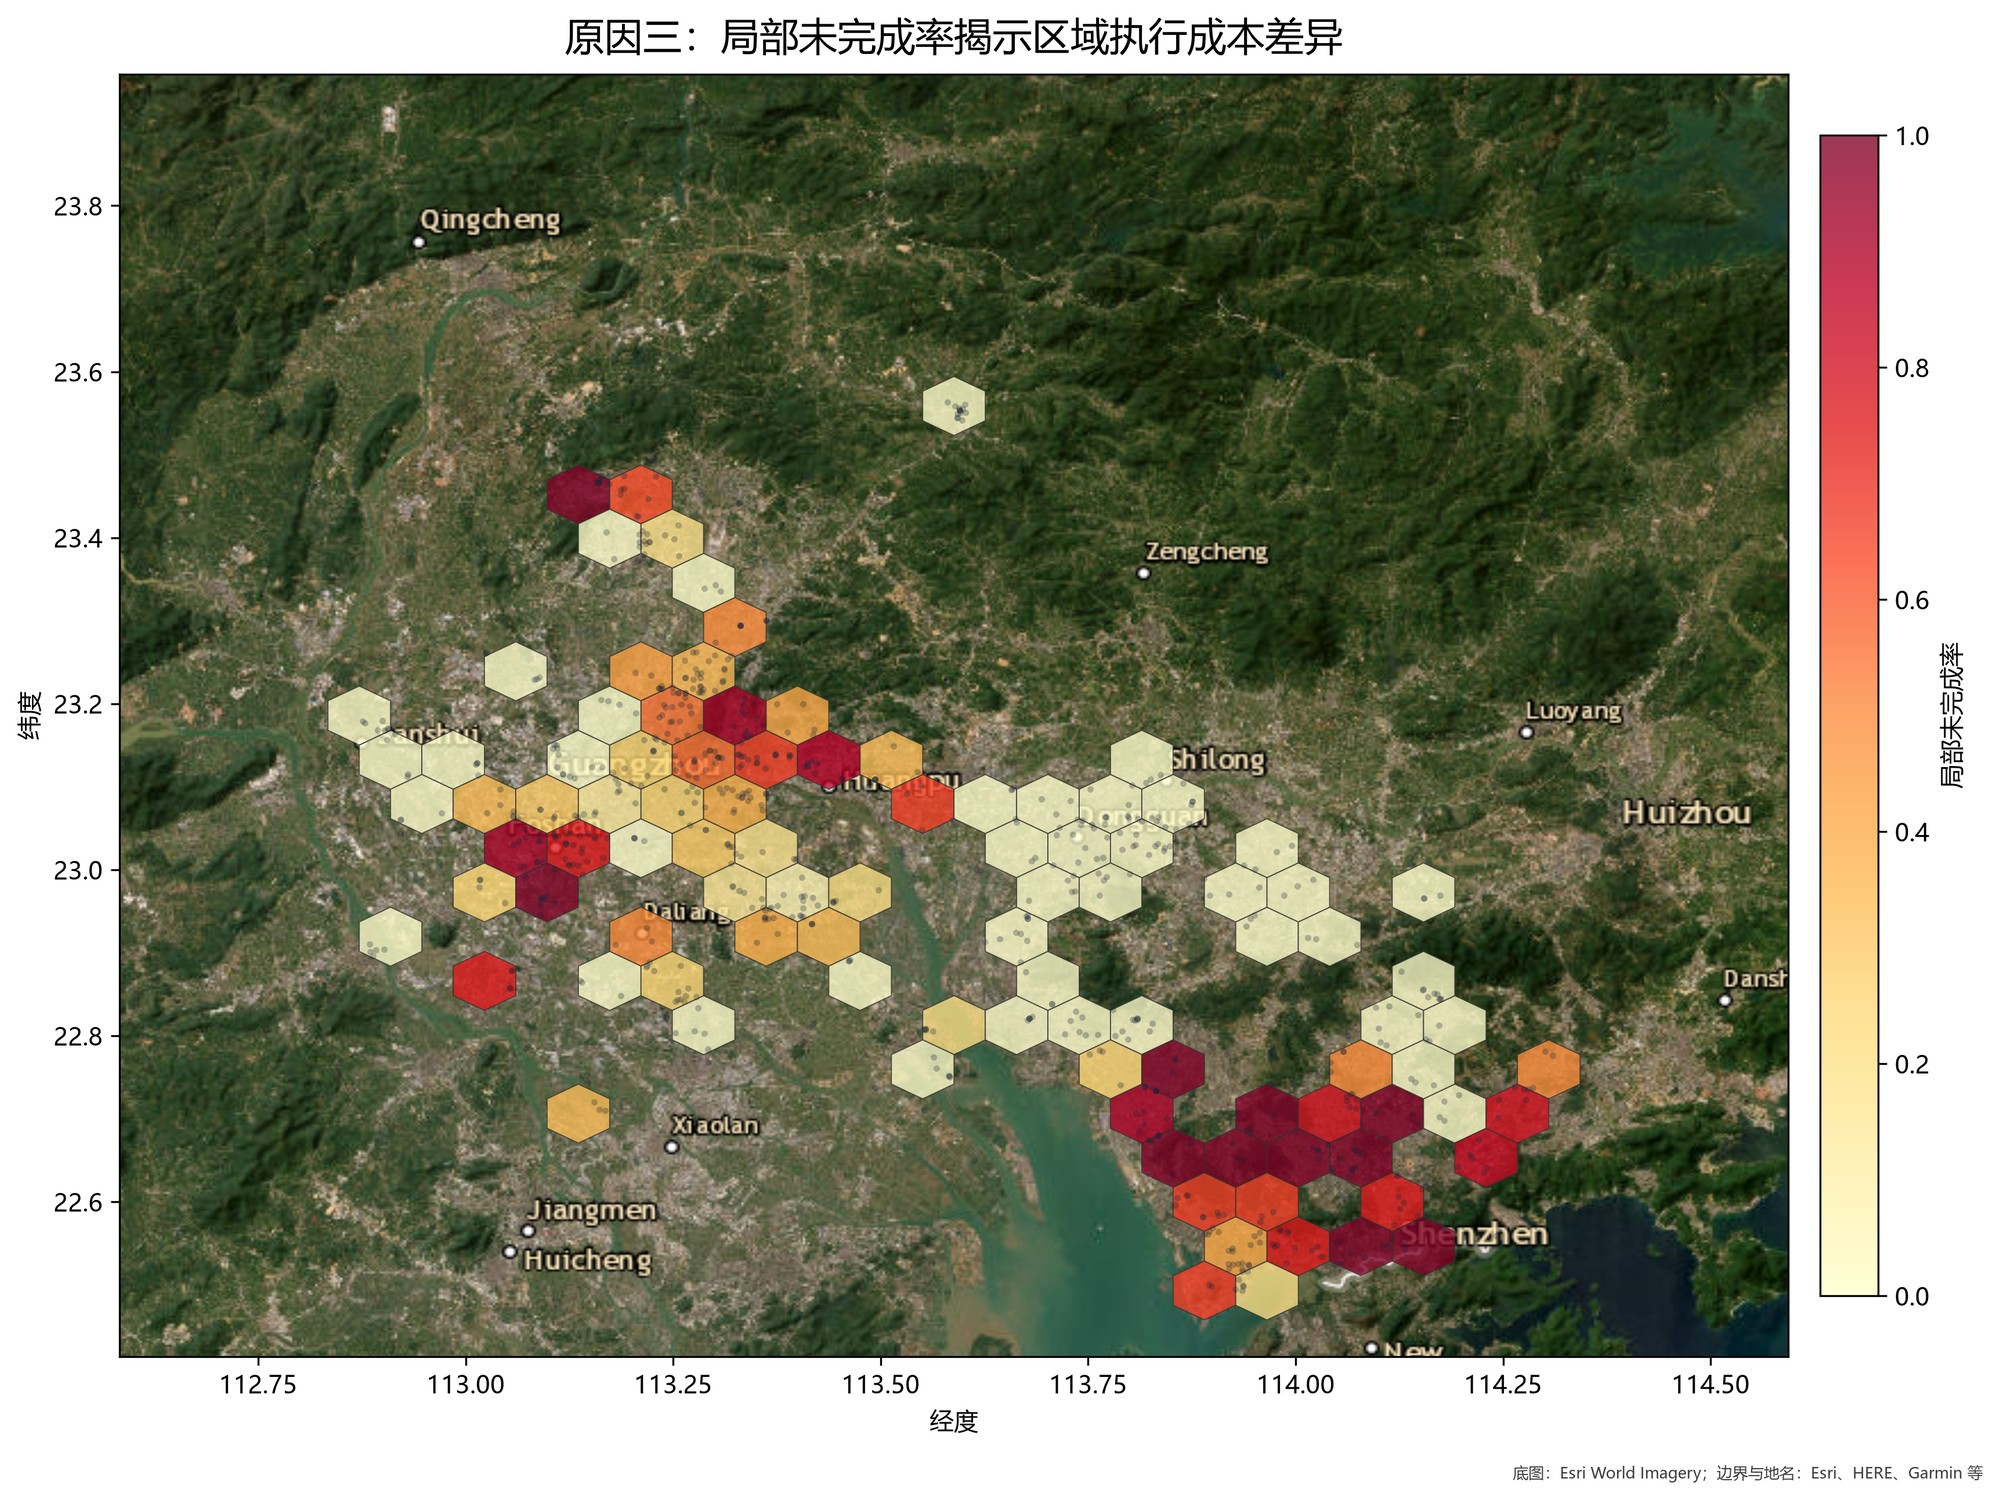
\includegraphics[width=0.96\textwidth]{../figures/fig-q1-region-v1.jpg}
  \caption{局部未完成率与区域综合执行成本差异}
  \label{fig:q1-region}
\end{figure}

\begin{table}[H]
  \centering
  \caption{问题一探索性空间分组的价格与完成率}
  \label{tab:q1-region}
  \begin{tabular}{lrrr}
    \toprule
    区域 & 任务数/个 & 平均价格/元 & 完成率/\% \\
    \midrule
    深圳附近 & 198 & 68.30 & 35.4 \\
    广州--佛山主要区域 & 386 & 68.77 & 60.6 \\
    广州北部 & 83 & 70.66 & 66.3 \\
    东莞附近 & 168 & 70.08 & 97.0 \\
    \bottomrule
  \end{tabular}
\end{table}

附件没有直接给出拥堵、停车或商户类型，故本文不把某一种城市成本写成已被数据证明的原因，而将其统称为区域固定效应或区域综合执行成本。该效应也可能包含会员活跃程度、任务发布时间及其他未观测因素。结论的可靠部分是：相近标价在不同区域对应的完成概率显著不同，原方案没有充分补偿这种稳定的空间差异。

区域效应并不严格服从行政边界，直接按城市统一加价会过于粗糙。问题二用5个空间聚类虚拟变量吸收平均差异，具体价格仍由任务级距离、邻域供需和价格响应决定，并设置区域服务下限以保护原有高完成区域。

\subsection{原因四：相邻任务存在竞争和选择替代}

按照式\eqref{eq:competition}将任务分为四组，结果见表\ref{tab:competition-group}。从低竞争组到高竞争组，完成率由66.7\%下降到59.8\%，同时平均价格由72.61元下降到67.19元。竞争效应的幅度小于价格分组和区域分组，但方向稳定，表明附近替代任务会降低当前任务的相对吸引力。

\begin{table}[H]
  \centering
  \caption{局部竞争强度分组的价格与完成率}
  \label{tab:competition-group}
  \begin{tabular}{lrrr}
    \toprule
    竞争强度 & 任务数/个 & 平均价格/元 & 完成率/\% \\
    \midrule
    低竞争 & 180 & 72.61 & 66.7 \\
    中低竞争 & 231 & 70.04 & 62.3 \\
    中高竞争 & 215 & 67.05 & 61.9 \\
    高竞争 & 209 & 67.19 & 59.8 \\
    \bottomrule
  \end{tabular}
\end{table}

图\ref{fig:q1-competition}显示，高竞争任务主要集中在广州中心和深圳任务密集区，并与未完成叉号明显重叠。会员面对多个邻近任务时会优先选择价格更高、距离更近或路线更方便的任务，低价任务因此被剩余。任务聚集同时具有“顺路完成”的便利效应和“争夺会员”的竞争效应；在问题一的单任务发布情形下，数据更支持竞争效应，而便利效应可在后续任务打包模型中利用。

\begin{figure}[H]
  \centering
  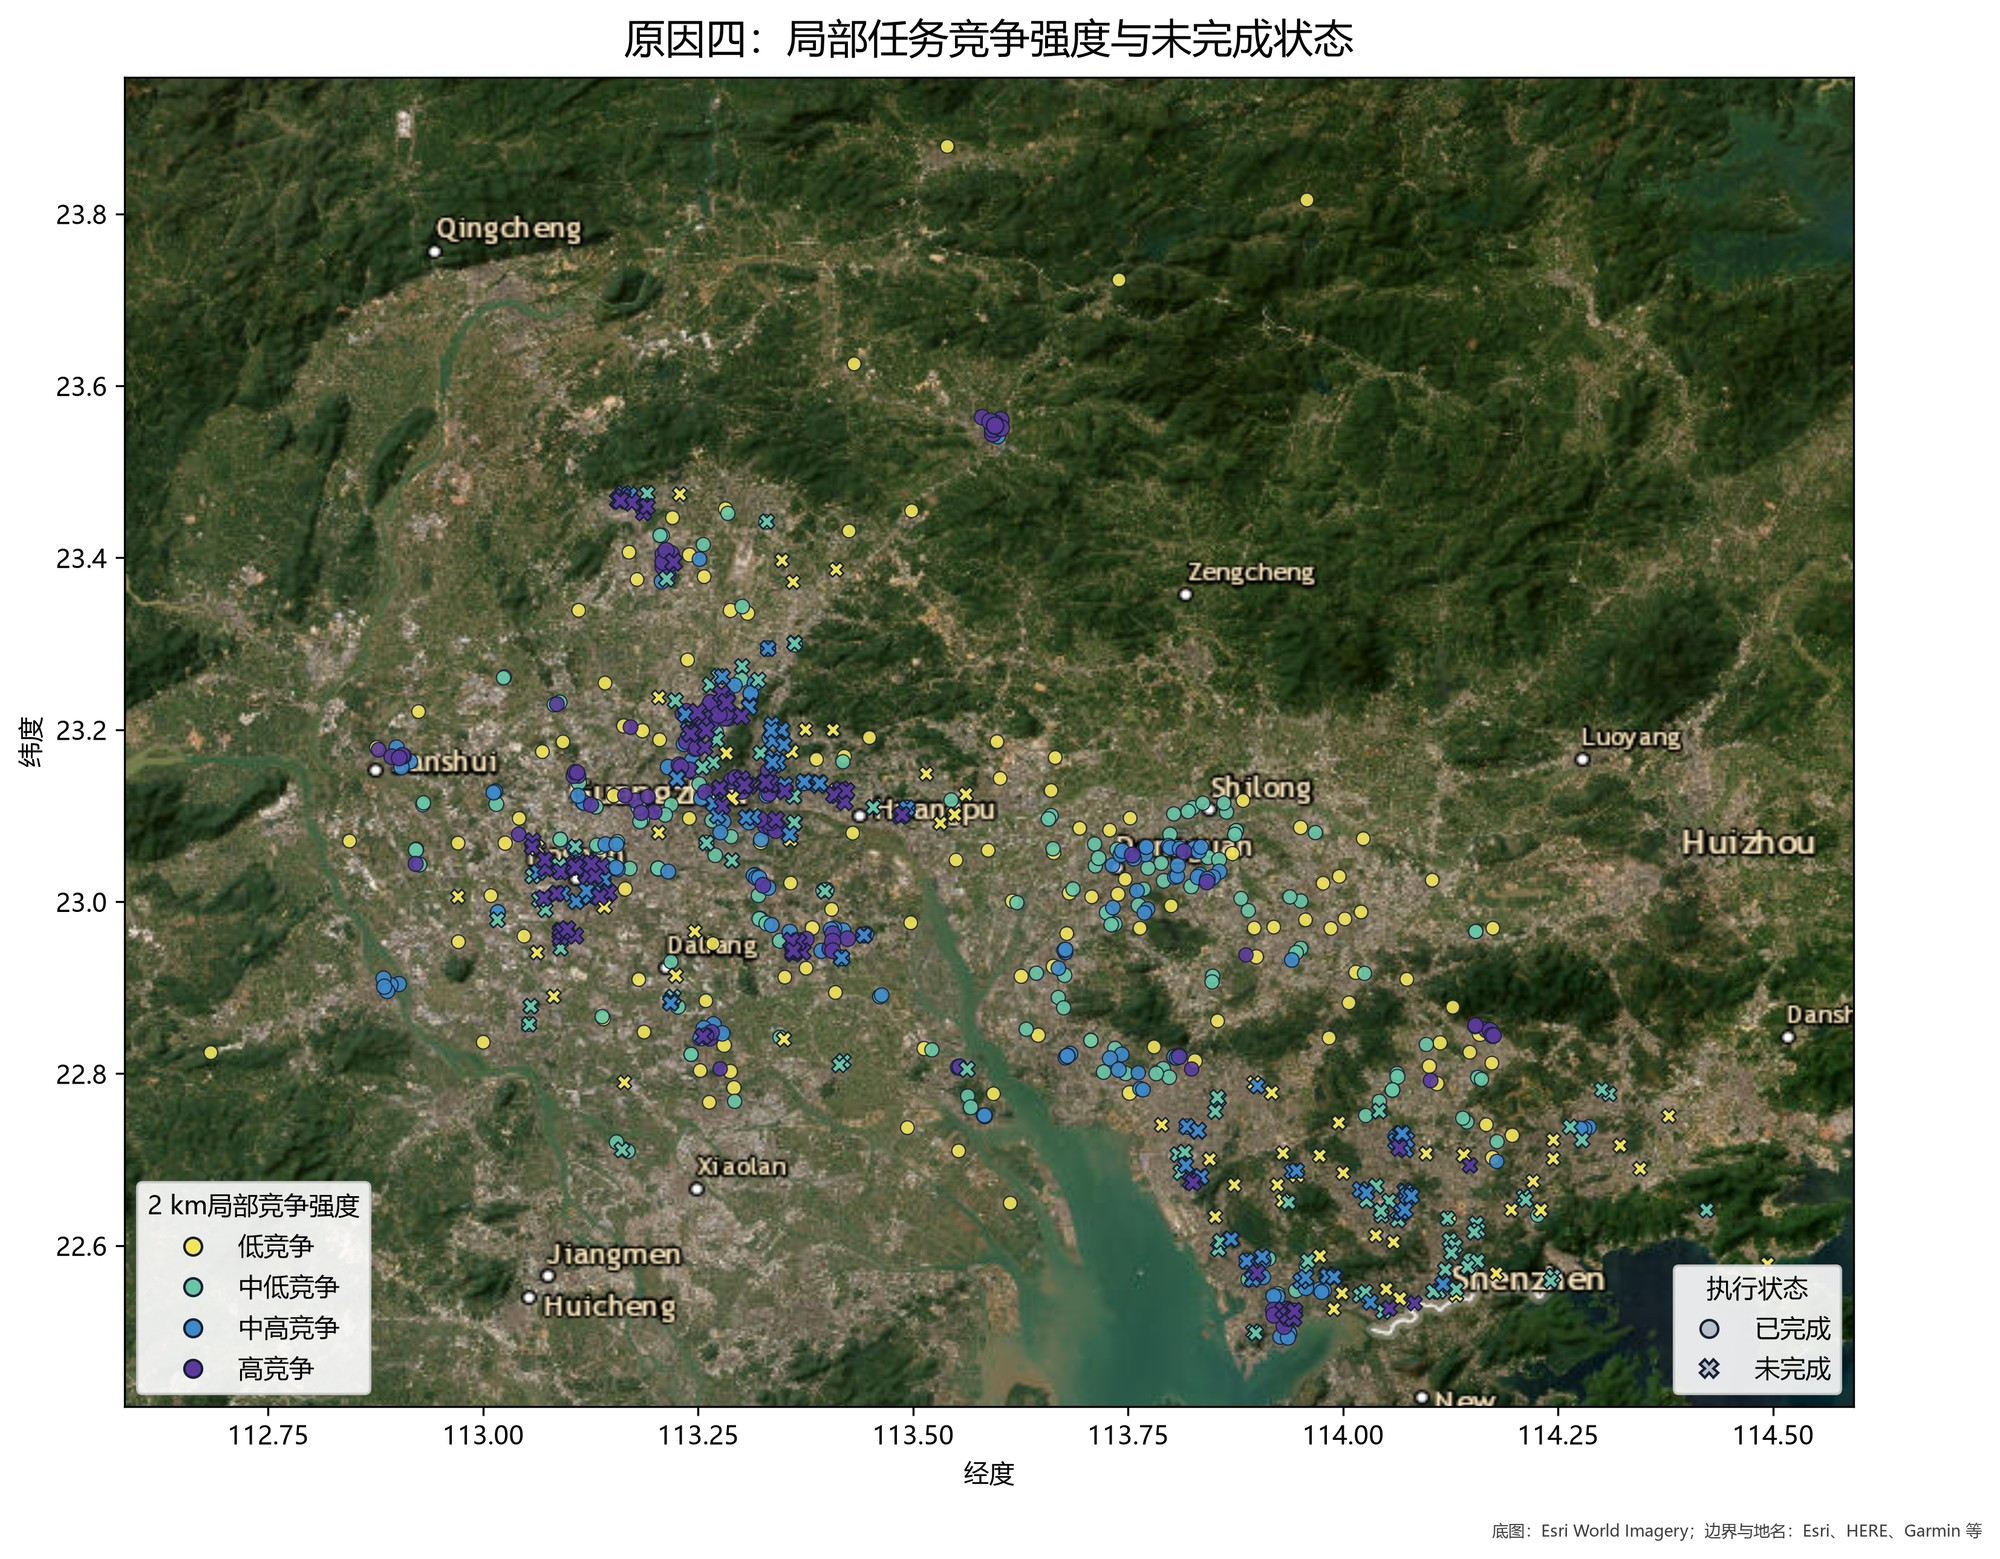
\includegraphics[width=0.96\textwidth]{../figures/fig-q1-competition-v1.jpg}
  \caption{局部任务竞争强度与未完成状态的空间分布}
  \label{fig:q1-competition}
\end{figure}

竞争强度同时考虑邻近任务数量和相对价格，比单纯计数更接近会员选择。分组完成率下降6.9个百分点，说明竞争不是唯一原因，但会与低价和区域难度共同放大失败风险。任务密度既可能造成选择替代，也可能产生顺路便利；单任务发布侧重前者，问题三则利用打包释放后者。

\subsection{多因素联合作用与因果边界}

四类因素并不独立：会员密集区往往同时低价且任务密集，单变量比较会混淆价格补偿、区域困难和供需竞争。多变量概率模型用于固定其他条件后比较候选价格，但历史数据并非随机调价试验，因此系数只用于预测和方案比较，不解释为严格因果效应。

\subsection{问题一结论}

四类原因形成连续的作用链：会员和任务向城区集中，平台据此判断任务容易被领取并降低标价；但注册会员并非全部有效，且密集任务相互竞争；城市综合执行成本又没有获得足够补偿，最终使低吸引力任务集中未完成。因此，原方案的问题不是缺少空间差异化，而是空间定价依据不完整。后续重新定价应以任务完成概率为中介，把有限成本优先投向价格响应较强的失败热点，而不是简单按会员数量或距离统一加价。

重新定价应允许“有升有降”：为深圳和广州热点加价，在不明显降低服务水平时适度下调东莞等高完成区域价格；加价后仍低概率的任务转入打包发布。由此确定问题二的成本重分配、调价边界和区域保护约束。

\section{问题二：成本约束下的任务重新定价}

\subsection{完成概率模型}

定义 $Y_i=1$ 表示任务完成，建立带 $L_2$ 正则化的 Logistic 模型
\begin{equation}
p_i(P)=\Pr(Y_i=1\mid P,\bm X_i)
=\frac{1}{1+\exp[-z_i(P)]},
\label{eq:logistic}
\end{equation}
其中
\begin{align}
z_i(P)=\;&\beta_0+\beta_1P+\beta_2D_i
+\beta_3\ln(1+N_i)+\beta_4\ln(1+G_i)\notag\\
&+\beta_5\ln(1+Q_i)+\beta_6\ln(1+H_i)
+\sum_{r=1}^{4}\gamma_rR_{ir}.
\label{eq:linear-predictor}
\end{align}
对计数和累计能力变量采用 $\ln(1+x)$ 变换，以降低右偏分布和极端值的影响。任务经纬度标准化后用 K-means 划分为5个空间区域，以吸收交通环境、商业类型和会员活跃程度等未直接观测的差异\cite{macqueen1967}。为保证反事实定价具有基本经济含义，约束标准化价格系数 $\beta_1\ge0$。

\subsubsection{变量作用与区域划分}

$D_i$ 表示最近潜在执行者的最低出行距离，$N_i$ 描述名义供给规模，$Q_i$ 和 $H_i$ 分别补充会员可承担任务量与信誉结构，$G_i$ 描述同一邻域的任务环境。将这些变量同时放入模型，可避免把“会员多但任务更多”的城区误判为供给绝对充足。模型没有直接使用历史完成状态构造加价标签，而是用全部任务共同估计系数，因此对已完成和未完成任务采用同一决策规则。

5个空间区域的中心大致对应广州中心及周边、东莞及周边、深圳及周边、佛山及广州西南部、广州北部。城市名称只用于结果解释，模型实际使用无序的聚类编号。聚类数过少会把深圳和东莞等差异明显的区域合并，过多则使每个区域样本不足、虚拟变量不稳定；5类在区域可解释性和样本量之间取得平衡。

区域虚拟变量用于吸收广域平均差异，而不是直接决定任务价格。候选价格变化时，区域项、距离项和供给项保持不变，所以 $p_i(P)$ 是同一任务沿价格轴的条件响应曲线。不同任务的曲线截距由空间环境决定：困难区域即使采用相同价格，预测完成概率仍可能较低；但由于Logistic曲线的斜率与当前概率有关，同样0.5元增量对不同任务产生的概率提升也不同。

\subsubsection{正则化与单调约束}

模型参数通过最小化带 $L_2$ 惩罚的负对数似然得到。连续变量经标准化后，惩罚系数取0.8，对截距不惩罚。正则化的作用是限制会员数量、限额和信誉等高度相关变量的系数幅度，降低小样本区域虚拟变量的波动。参数采用带边界的数值优化求解，价格系数下界为0，其余系数不预设方向。

单调约束是新定价能够成立的必要条件。若完全按照观察性数据无约束拟合，平台原先对困难任务加价可能使价格系数被反向混杂，出现“提高价格反而降低完成概率”的局部解释；把这种关系用于反事实优化会产生不符合会员收益逻辑的降价建议。非负约束并不能消除全部混杂，但至少保证方案在其他特征不变时不会因加价而降低预测完成率。

模型在835条历史样本上的初步拟合指标见表\ref{tab:model-fit}。训练集 AUC 为0.7995，Brier 得分为0.1732，标准化价格系数为0.2430。原价格下预测完成数为522.0004，与实际完成数522几乎一致，说明总体概率均值已校准。需要强调的是，这两项性能为训练集指标，不代表空间外推能力；最终结果因此只作为方案比较的预测值\cite{hosmer2013}。

\begin{table}[H]
  \centering
  \caption{任务完成概率模型的初步拟合指标}
  \label{tab:model-fit}
  \begin{tabular}{lr}
    \toprule
    指标 & 数值 \\
    \midrule
    样本数/个 & 835 \\
    历史实际完成率/\% & 62.51 \\
    训练集 AUC & 0.7995 \\
    训练集 Brier 得分 & 0.1732 \\
    标准化价格系数 & 0.2430 \\
    原方案预测完成数/个 & 522.0004 \\
    原方案预测完成率/\% & 62.5150 \\
    \bottomrule
  \end{tabular}
\end{table}

\subsubsection{拟合指标的解释边界}

AUC衡量模型把完成任务排在未完成任务之前的能力，0.7995说明模型对任务难易具有较好的区分度；Brier得分同时考察概率偏差和校准程度，数值越小越好。原方案预测完成数与真实完成数相等，只能说明总体均值一致，不能保证每个区域和每个任务都准确。尤其在空间数据中，相邻任务共享会员和道路环境，随机划分训练集与测试集可能造成信息泄漏。

因此，本文把训练指标用于确认模型具备进入优化的基本辨别能力，而不把它们写成最终泛化性能。新方案比较全部在同一模型、同一批任务和同一成本口径下进行，重点是相对变化而非声称绝对预测无误。正式上线前应按空间块留出区域进行交叉验证，并对每个区域的预测概率进行可靠性曲线校准。

\subsection{候选价格与成本口径}

对每个任务设置0.5元步长的候选价格集合
\begin{equation}
\mathcal P_i=\{P_{ik}:65\le P_{ik}\le85,\;
|P_{ik}-P_i|\le8\}.
\label{eq:candidate}
\end{equation}
该范围一方面遵守历史价格上下界，另一方面避免原价65元的任务直接跳到85元。对任一候选价格，任务 $i$ 的预计支付金额为
\begin{equation}
c_{ik}=P_{ik}p_i(P_{ik}).
\label{eq:expected-cost-item}
\end{equation}
原方案在同一模型口径下的预计支付金额为
\begin{equation}
C_0=\sum_iP_ip_i(P_i)=36444.28\ \text{元}.
\label{eq:baseline-cost}
\end{equation}
推荐方案允许成本最多增加15\%，故 $C_{\max}=1.15C_0=41910.92$ 元。历史实际支付金额为36446元，与式\eqref{eq:baseline-cost}相差很小，可作为总体校准的辅助证据。

将 $\mathcal P_i$ 中各价格代入式\eqref{eq:logistic}和式\eqref{eq:expected-cost-item}，形成逐任务概率--成本矩阵。每项任务最多33个候选点，定价问题由此转化为有限二元选择；0.5元网格与原价格精度一致，也使候选价格可直接发布和追溯。

全部标价总额 $\sum_iP_i$ 表示所有任务均完成时的最大承诺金额，却不能代表历史实际支出。若一个高价任务完成概率很低，平台的预计支出远小于标价；反之，低价但高完成概率任务会稳定产生支付。使用 $\sum_iP_ip_i(P_i)$ 可以同时反映价格和完成概率，并使新旧方案具有相同模型口径。

该口径未包含审核、客服和失败重发等平台成本，因此只作为可由附件核算的任务酬金预算，不代表全部经营成本。

预计支付的另一作用是避免把“提高完成率”与“提高全部标价”混为一谈。优化只在任务实际完成时计入报酬，能够把成本从高完成、低边际收益任务转移给低完成、高边际收益任务。与此同时，完成率上升还可能减少失败重发和延期成本，故当前口径对方案收益的评价偏保守；正文同时报告平均价格、预计支付和新增完成数，不用单一成本指标替代全部经营含义。

\subsection{多选择背包定价模型}

令二元变量 $x_{ik}=1$ 表示为任务 $i$ 选择候选价格 $P_{ik}$。每个任务必须且只能选择一个价格，纯完成率最优模型为
\begin{align}
\max\quad &\sum_i\sum_{k\in\mathcal P_i}p_i(P_{ik})x_{ik},
\label{eq:milp-objective}\\
\text{s.t.}\quad
&\sum_{k\in\mathcal P_i}x_{ik}=1,\quad \forall i, \label{eq:one-price}\\
&\sum_i\sum_{k\in\mathcal P_i}c_{ik}x_{ik}\le C_{\max}, \label{eq:cost-constraint}\\
&x_{ik}\in\{0,1\}. \label{eq:binary}
\end{align}
这是一个多选择背包形式的混合整数线性规划，可由分支定界求得全局最优解\cite{dantzig1957}。式\eqref{eq:one-price}对应“一项任务一个标价”，式\eqref{eq:cost-constraint}对应预计支付预算，候选集合已包含价格范围和单任务最大调价限制。

目标函数等于预计完成数，不把概率视为确定标签，也不强制所有任务达到统一阈值。模型使用SciPy的 \texttt{milp} 接口和HiGHS求解器，两类MILP均返回最优状态，最优性间隙约为 $10^{-6}$。

为验证求解结构，另设计边际效率贪心算法。当任务价格从 $P$ 增加到 $P+0.5$ 时，定义
\begin{equation}
E_i(P)=
\frac{p_i(P+0.5)-p_i(P)}
{(P+0.5)p_i(P+0.5)-Pp_i(P)}.
\label{eq:marginal-efficiency}
\end{equation}
贪心算法从各任务最低允许价格出发，按 $E_i(P)$ 从高到低接受不违反预算的0.5元增量，作为快速基线。其逐步决策不保证多选择背包的全局最优，因此最终与精确MILP比较。

\subsection{价格稳定性与区域服务约束}

纯完成率最优可能把大量任务推到 $\pm8$ 元边界，并通过降低高完成区域价格释放预算。为提高实施稳定性，在目标中加入价格调整平方惩罚：
\begin{equation}
\max\ \sum_i\sum_k
\left[p_i(P_{ik})-\mu\left(\frac{P_{ik}-P_i}{8}\right)^2\right]x_{ik},
\qquad \mu=0.015.
\label{eq:practical-objective}
\end{equation}
系数 $\mu$ 为经验稳定性参数，其作用不是改变预算，而是在完成概率接近时优先选择调价幅度较小的方案。

对每个空间区域 $r$，再限制新方案区域平均完成率最多下降1个百分点：
\begin{equation}
\frac{1}{n_r}\sum_{i\in r}\sum_kp_i(P_{ik})x_{ik}
\ge \bar p_r^{\,0}-0.01,
\label{eq:region-floor}
\end{equation}
其中 $\bar p_r^{\,0}$ 为原方案在区域 $r$ 的平均预测完成率。由式\eqref{eq:practical-objective}与式\eqref{eq:region-floor}得到的方案称为实用 MILP，并作为最终推荐方案。

平方惩罚仅在完成概率接近时偏向较小调价，不改变预算；区域下限则防止优化持续压低东莞等高完成区域的价格。故精确MILP给出完成数上限，实用MILP以少量目标损失换取价格与区域结果的稳定性。

惩罚项按最大调价8元归一化，取值不超过0.015，因此只对概率非常接近的候选价重新排序。区域服务下限允许各区域平均预测完成率最多下降1个百分点，既保留预算转移空间，又阻止某一区域为全局目标承担过多损失。这两个参数均为实施偏好而非客观常数，必须结合最终边界任务数和区域结果检查其实际影响。

\subsection{总体结果与算法比较}

表\ref{tab:milp-compare}比较原方案、边际效率贪心、精确 MILP 和实用 MILP。精确 MILP 比贪心方案只多0.0010个预计完成任务，预测完成率仅高约0.0001个百分点，说明当前概率曲线下边际收益近似递减，贪心算法已非常接近全局最优。求解器进一步给出最优状态和约 $10^{-6}$ 的最优性间隙。

\begin{table}[H]
  \centering
  \caption{原方案与三种重新定价方案的总体结果}
  \label{tab:milp-compare}
  \resizebox{\textwidth}{!}{%
  \begin{tabular}{lrrrrrr}
    \toprule
    方案 & 平均价格/元 & 预计支付/元 & 预测完成数/个 &
    预测完成率/\% & 平均绝对调价/元 & 边界任务数/个 \\
    \midrule
    原方案 & 69.1108 & 36444.28 & 522.0004 & 62.5150 & 0 & 0 \\
    贪心方案 & 73.5778 & 41910.67 & 574.5378 & 68.8069 & 6.5629 & 557 \\
    精确 MILP & 73.5778 & 41910.83 & 574.5387 & 68.8070 & 6.5653 & 557 \\
    实用 MILP & 73.6144 & 41910.85 & 573.9560 & 68.7372 & 6.0737 & 433 \\
    \bottomrule
  \end{tabular}}
\end{table}

实用 MILP 相比贪心方案仅减少0.58个预计完成任务、降低0.07个百分点，但边界任务减少124个，下降22.3\%；平均绝对调价减少0.49元，定价65元的任务由156个减少到115个。方案中633个任务提价、175个任务降价、27个任务不变，只有24个任务达到85元上限。由此可见，稳定性修正以极小的完成率损失换来了更平滑的价格结构。

\subsection{区域价格转移与实施含义}

表\ref{tab:regional-result}给出实用 MILP 的区域结果。广州中心、深圳、佛山及广州西南部是主要加价区域，预测完成率分别提高8.84、9.28和7.20个百分点；东莞原预测完成率高达94.88\%，平均价格适度下降3.50元后仍保持94.15\%，且下降0.73个百分点，没有触发区域服务下限。模型由此把部分预算从高完成概率区域转向问题一识别出的失败热点。

\begin{table}[H]
  \centering
  \caption{实用MILP方案的区域价格与预测完成率变化}
  \label{tab:regional-result}
  \resizebox{\textwidth}{!}{%
  \begin{tabular}{lrrrrr}
    \toprule
    区域 & 任务数/个 & 原均价/元 & 新均价/元 &
    原完成率/\% & 新完成率/\% \\
    \midrule
    广州中心及周边 & 213 & 67.35 & 74.37 & 56.42 & 65.26 \\
    东莞及周边 & 185 & 69.81 & 66.32 & 94.88 & 94.15 \\
    深圳及周边 & 200 & 68.35 & 76.11 & 36.24 & 45.52 \\
    佛山及广州西南部 & 172 & 70.45 & 76.48 & 62.78 & 69.98 \\
    广州北部 & 65 & 71.68 & 76.65 & 70.52 & 75.95 \\
    \bottomrule
  \end{tabular}}
\end{table}

深圳区域虽然平均价格提高到76.11元，预测完成率仍只有45.52\%，说明该区域的困难不能完全依靠单任务加价消除。对于达到调价上限后仍保持低完成概率的任务，更合适的后续措施是改变发布方式，例如将相邻任务打包以降低平均出行成本，而不是继续突破85元上限。

广州中心平均加价7.02元，完成率提高8.84个百分点；东莞平均降价3.50元，完成率仅下降0.73个百分点。该结果体现成本由低边际收益区域向失败热点转移，而非普遍涨价。区域名称只用于解释聚类中心，边界任务仍按逐任务特征定价。

\subsection{预算敏感性分析}

表\ref{tab:scenarios}展示不同预计成本增幅和单任务调价上限下的预测完成率。成本中性重分配即可把预测完成率从62.52\%提高到63.54\%；成本上限依次提高到5\%、10\%和15\%时，$\pm5$ 元方案的完成率为65.32\%、66.75\%和67.19\%。允许 $\pm8$ 元调整后，10\%和15\%预算对应67.36\%和68.81\%。若进一步采用20\%预算和 $\pm10$ 元上限，完成率可达到70.50\%，但预计支付还需增加约1822元，且价格变化更剧烈。

\begin{table}[H]
  \centering
  \caption{不同预算与调价幅度情景的预测结果}
  \label{tab:scenarios}
  \begin{tabular}{lrrrr}
    \toprule
    情景 & 成本增幅/\% & 最大调价/元 & 平均价格/元 & 预测完成率/\% \\
    \midrule
    成本中性 & 0 & 5 & 69.20 & 63.54 \\
    平衡方案 & 5 & 5 & 70.64 & 65.32 \\
    增强方案 & 10 & 5 & 72.13 & 66.75 \\
    增强方案 & 15 & 5 & 73.95 & 67.19 \\
    宽幅方案 & 10 & 8 & 72.11 & 67.36 \\
    宽幅方案 & 15 & 8 & 73.58 & 68.81 \\
    完成优先 & 20 & 10 & 75.03 & 70.50 \\
    \bottomrule
  \end{tabular}
\end{table}

\begin{figure}[htbp]
  \centering
  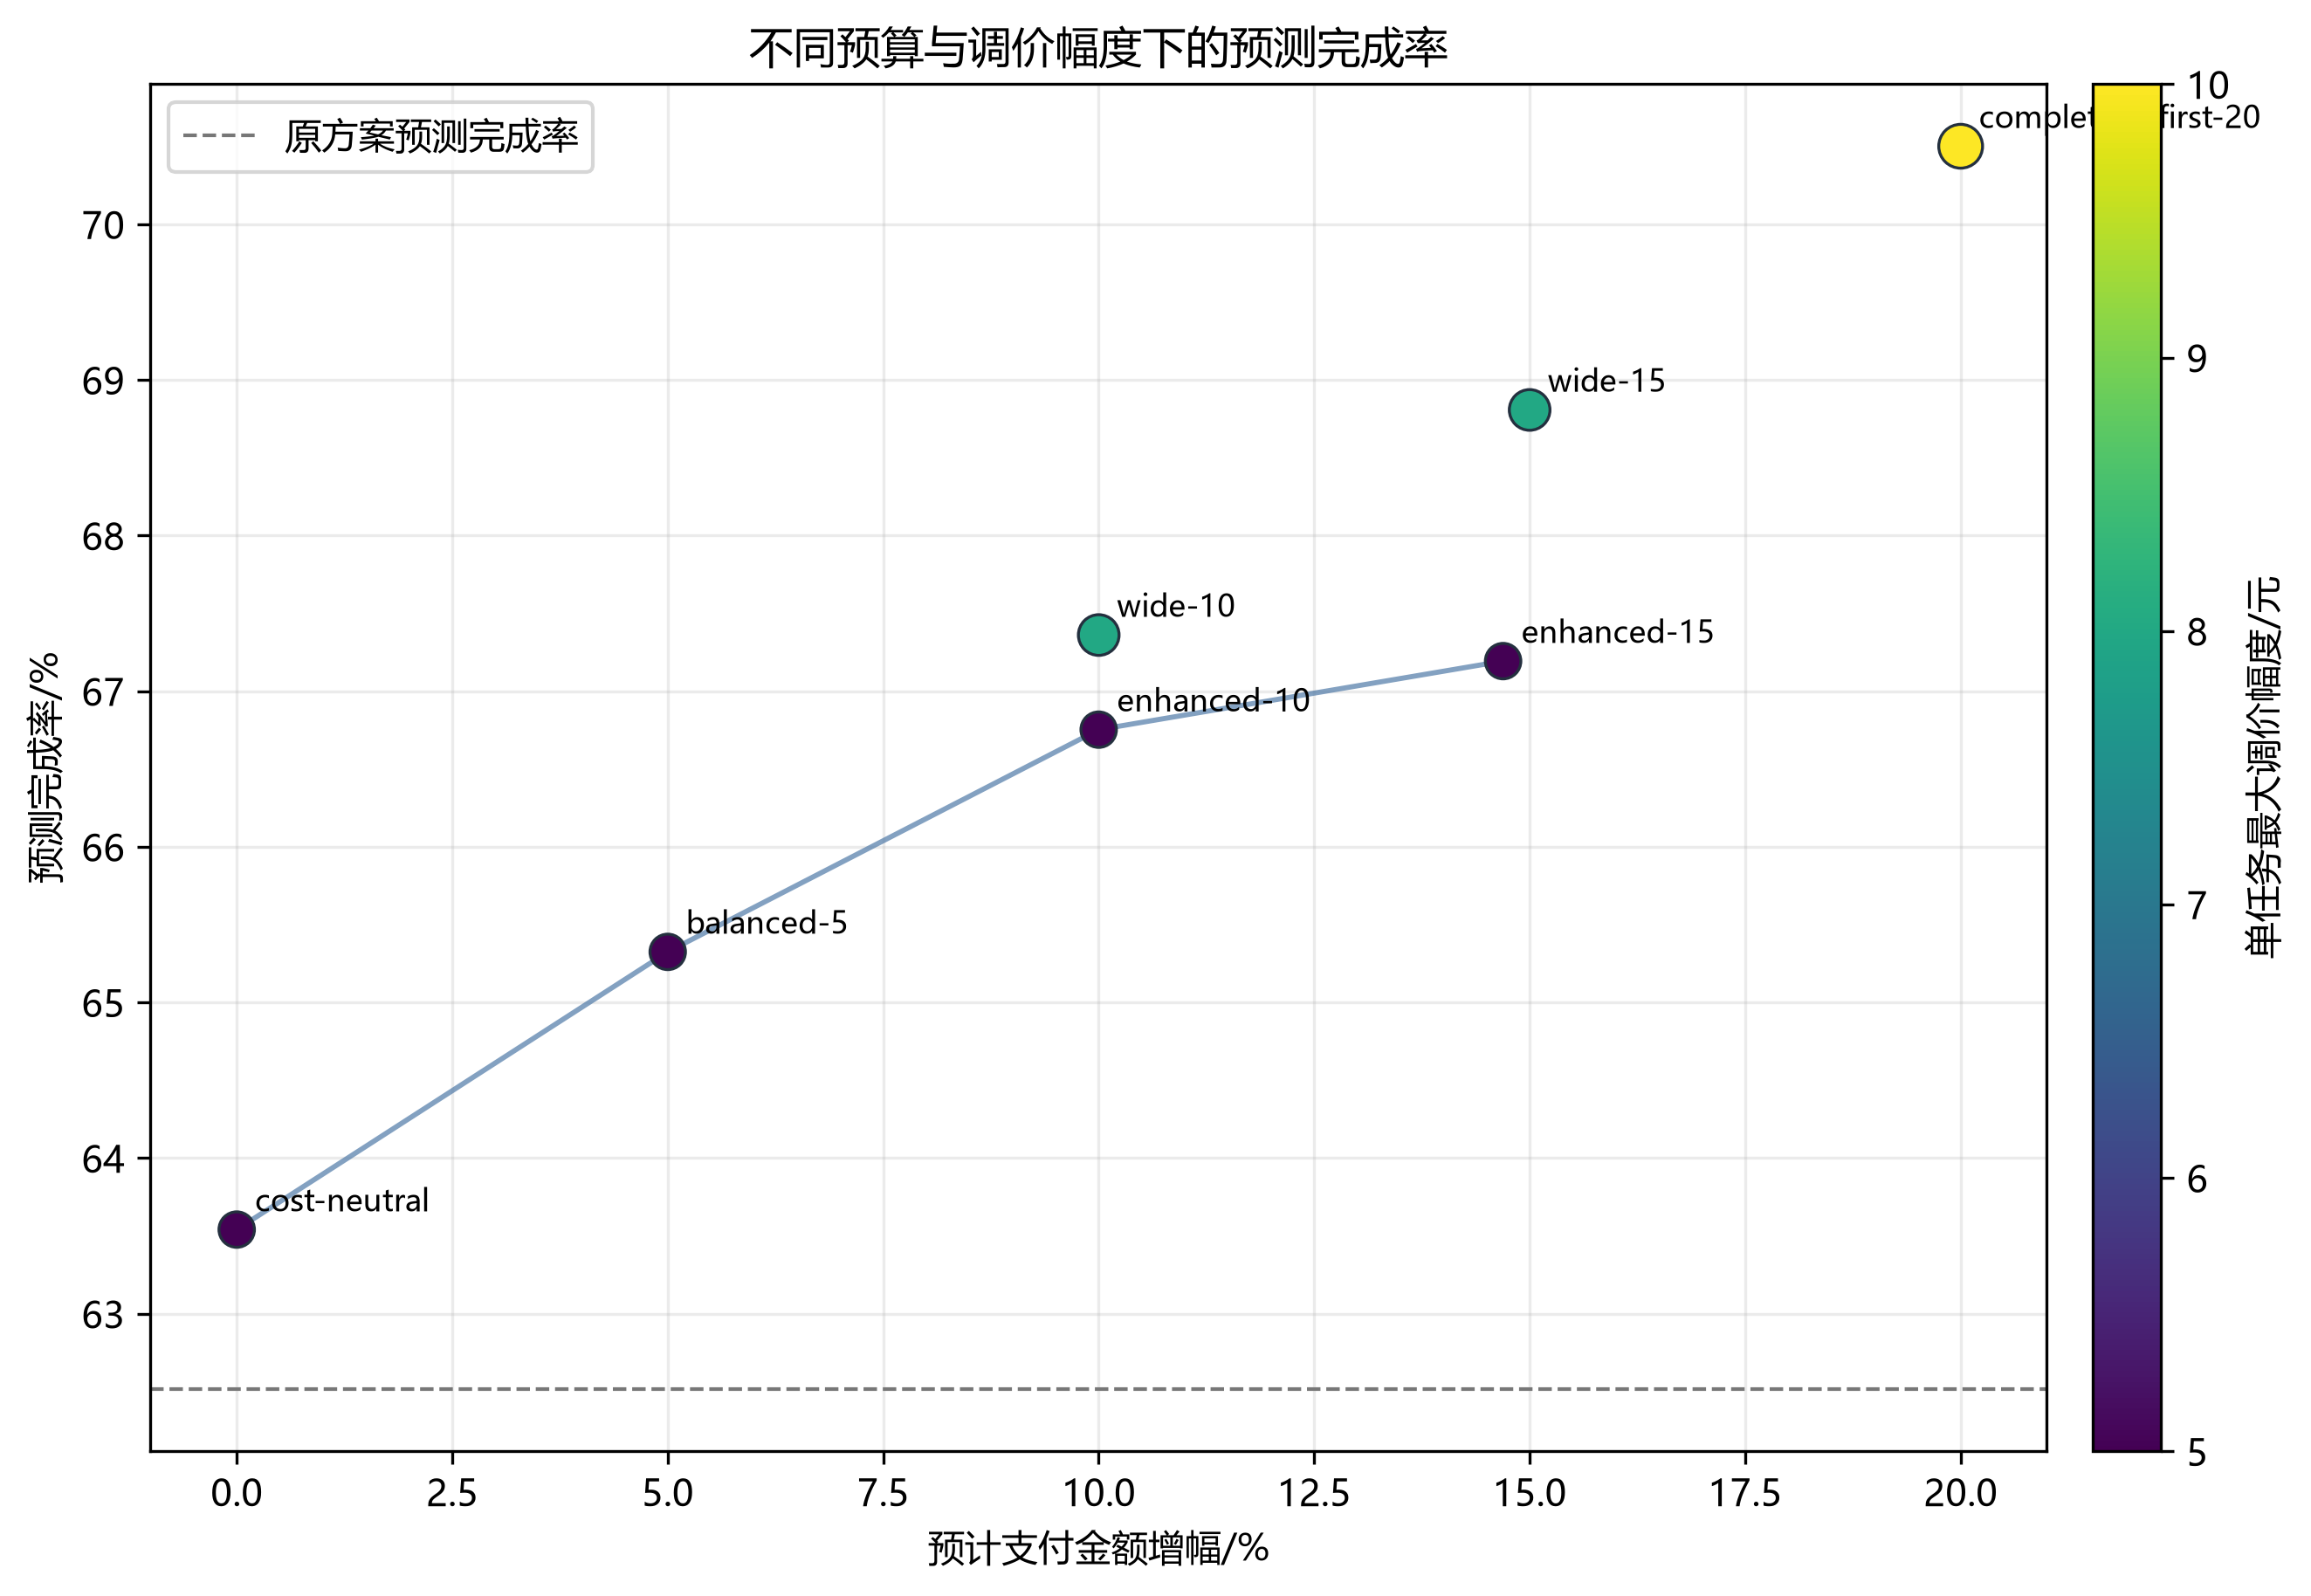
\includegraphics[width=0.86\textwidth]{../figures/fig-q2-scenarios-v1.png}
  \caption{不同预算与调价幅度下的预测完成率}
  \label{fig:q2-scenarios}
\end{figure}

表\ref{tab:scenarios}显示，成本由10\%增至15\%仍有明显收益，增至20\%后边际改善趋缓；同预算下放宽调价上限有利于补偿失败热点。成本中性重分配也能提高约8.56个预计完成任务，但不足以处理深圳等区域的系统性低价，故推荐15\%预算、$\pm8$元方案。该分析检验的是优化约束，而非统计参数不确定性。

在10\%预算下，$\pm8$元方案比$\pm5$元方案高0.61个百分点；在15\%预算下差距扩大至1.61个百分点，说明部分热点需要超过5元的补偿。但20\%预算与$\pm10$元上限只比推荐方案再提高1.69个百分点，平均价格却升至75.03元。若要检验统计不确定性，还需在空间分块重采样中重复拟合概率模型，统计推荐价格的选择频率和区间。

\subsection{结果一致性与边界检查}

原方案预测完成数522.0004，与实际522基本一致；实用MILP预计支付41910.85元，未超过41910.92元上限，835项任务均唯一选价且调价位于$[-8,8]$元。东莞完成率下降0.73个百分点，满足1个百分点区域下限。精确MILP仅比贪心多0.0010个预计完成任务；实用MILP少0.5828个，却减少124个边界任务，量化了稳定性代价。

\subsection{问题二结论}

在65--85元价格范围、0.5元步长、单任务调整不超过 $\pm8$ 元且预计支付成本不超过原方案115\%的条件下，实用 MILP 将平均价格调整为73.61元，预计支付金额为41910.85元，预测完成数为573.96个，预测完成率为68.74\%，相对原方案增加51.96个预计完成任务。该方案重点补偿深圳、广州中心和佛山部分失败热点，同时保持东莞等高完成区域的服务水平。由于结果来自历史数据上的反事实预测，正式实施时应先进行小范围试运行，并用真实领取、拒绝、完成和取消记录重新校准价格响应。\aimark{4}

\section{问题三：任务打包发布与联合定价}

\subsection{打包对象与空间路线}

问题二仍有一批任务在达到调价边界后预测完成概率低于0.5，说明继续采用单任务加价的边际收益有限。另一方面，密集区的相邻任务既会竞争会员，也可能共享一次出行。若把空间紧凑的任务联合发布，会员获得较高的总酬金，并能在一次路线中完成多项工作，平台便可把“任务竞争”转化为“路线协同”。因此本问不预先指定哪些任务必须打包，而是让单任务方案与候选任务包在同一优化模型中竞争。

以问题二实用MILP结果为基线，定义核心困难任务集合
\begin{equation}
 \mathcal D=\{i:p_i'<0.5,\ |P_i'-P_i|\geq 8\},
 \label{eq:core}
\end{equation}
其中$p_i'$和$P_i'$分别为问题二推荐价格下的完成概率和价格。核心任务可与同一区域、距离不超过1 km且$p_j'<0.75$的顺路任务组合。每个候选包含2--5个任务，并至少包含一个核心任务。这一筛选把打包资源集中于单任务方案难以处理的对象，同时允许中等概率任务作为路线锚点。

经纬度在珠三角小范围内转换为公里平面坐标。对任务包$g$的任务集合$S_g$，用最小生成树长度$L_g$近似访问全部任务所需的内部路线，定义
\begin{equation}
 \bar d_g=\frac{L_g}{\max(|S_g|-1,1)},\qquad
 H_g=\max\left(0,1-\frac{\bar d_g}{1\ {\rm km}}\right).
 \label{eq:compact}
\end{equation}
$H_g$越大表示包越紧凑。与简单使用包内最大距离相比，最小生成树同时利用所有任务点的连接关系，且不要求预先指定访问顺序。它低估了真实道路行程，因此只用于候选筛选和相对比较，不能被解释为实际里程。

\subsection{任务包完成概率}

附件没有历史打包发布记录，不能直接拟合包级完成率。本文以问题二单任务概率为基础，构造透明的结构修正，而不把其伪装为观测结果。设包平均单任务价格为$A_{gk}$，价格倍率$\rho_k\in\{0.85,0.90,\ldots,1.15\}$，则总包价为$B_{gk}=|S_g|A_{gk}$。先取包内单任务logit均值，再加入价格、规模、紧凑度和执行负担：
\begin{align}
 \eta_{gk}={}&\frac{1}{|S_g|}\sum_{i\in S_g}\operatorname{logit}(p_i')
 s_g(A_{gk}-\bar P_g')+0.42\ln |S_g|+0.55H_g \nonumber\\
 &+0.12(1-r_g)-0.07(|S_g|-1)-0.10\max(0,L_g-1),\\
 p_{gk}={}&(1+\exp(-\eta_{gk}))^{-1}.
 \label{eq:bundle-prob}
\end{align}
其中$s_g$由包内任务在问题二调价前后的logit变化率估计并截断到$[0.02,0.20]$，$r_g$为核心任务占比。对数规模项描述总酬金增加但边际吸引力递减；紧凑度奖励路线共享；任务数和超出1 km的路线长度形成负担惩罚。系数属于情景参数，结论必须结合0\%、1\%、2\%预算情景比较，实际部署后再由包领取数据校准。

\subsection{单任务与任务包联合MILP}

令$x_{ik}$表示任务$i$单独发布并选择价格$P_{ik}$，$z_{gk}$表示选择任务包$g$及价格$B_{gk}$。每个任务必须且只能出现一次：
\begin{equation}
 \sum_kx_{ik}+\sum_{g:i\in S_g}\sum_kz_{gk}=1,\quad \forall i.
 \label{eq:cover}
\end{equation}
在预计支付预算$C_{\max}$下最大化预计完成任务数：
\begin{align}
 \max\quad &\sum_i\sum_k p_{ik}x_{ik}
 +\sum_g\sum_k |S_g|p_{gk}z_{gk},\\
 {\rm s.t.}\quad&
 \sum_i\sum_k P_{ik}p_{ik}x_{ik}
 +\sum_g\sum_k B_{gk}p_{gk}z_{gk}\leq C_{\max},\nonumber\\
 &x_{ik},z_{gk}\in\{0,1\}.
 \label{eq:bundle-milp}
\end{align}
所有概率和预计支付在求解前计算，因此模型保持线性。共形成19387个单任务价格候选、1407个包价格候选，共20794个二元变量；HiGHS在三种预算情景下均获得约$10^{-6}$的最优性间隙。覆盖约束同时排除了任务遗漏、重复打包和单包并行发布。

\subsection{结果与影响分析}

\begin{table}[H]
\centering
\caption{问题三联合打包定价的预算情景结果}
\begin{tabular}{lrrrr}
\toprule
方案 & 预计支付/元 & 预计完成数 & 完成率/\% & 较问题二增加/个\\
\midrule
问题二实用MILP & 41910.85 & 573.96 & 68.74 & --\\
打包，预算不变 & 41910.79 & 584.55 & 70.01 & 10.60\\
打包，预算增加1\% & 42329.90 & 587.69 & 70.38 & 13.73\\
打包，预算增加2\% & 42749.00 & 590.76 & 70.75 & 16.80\\
\bottomrule
\end{tabular}
\label{tab:q3-results}
\end{table}

\begin{figure}[H]
\centering
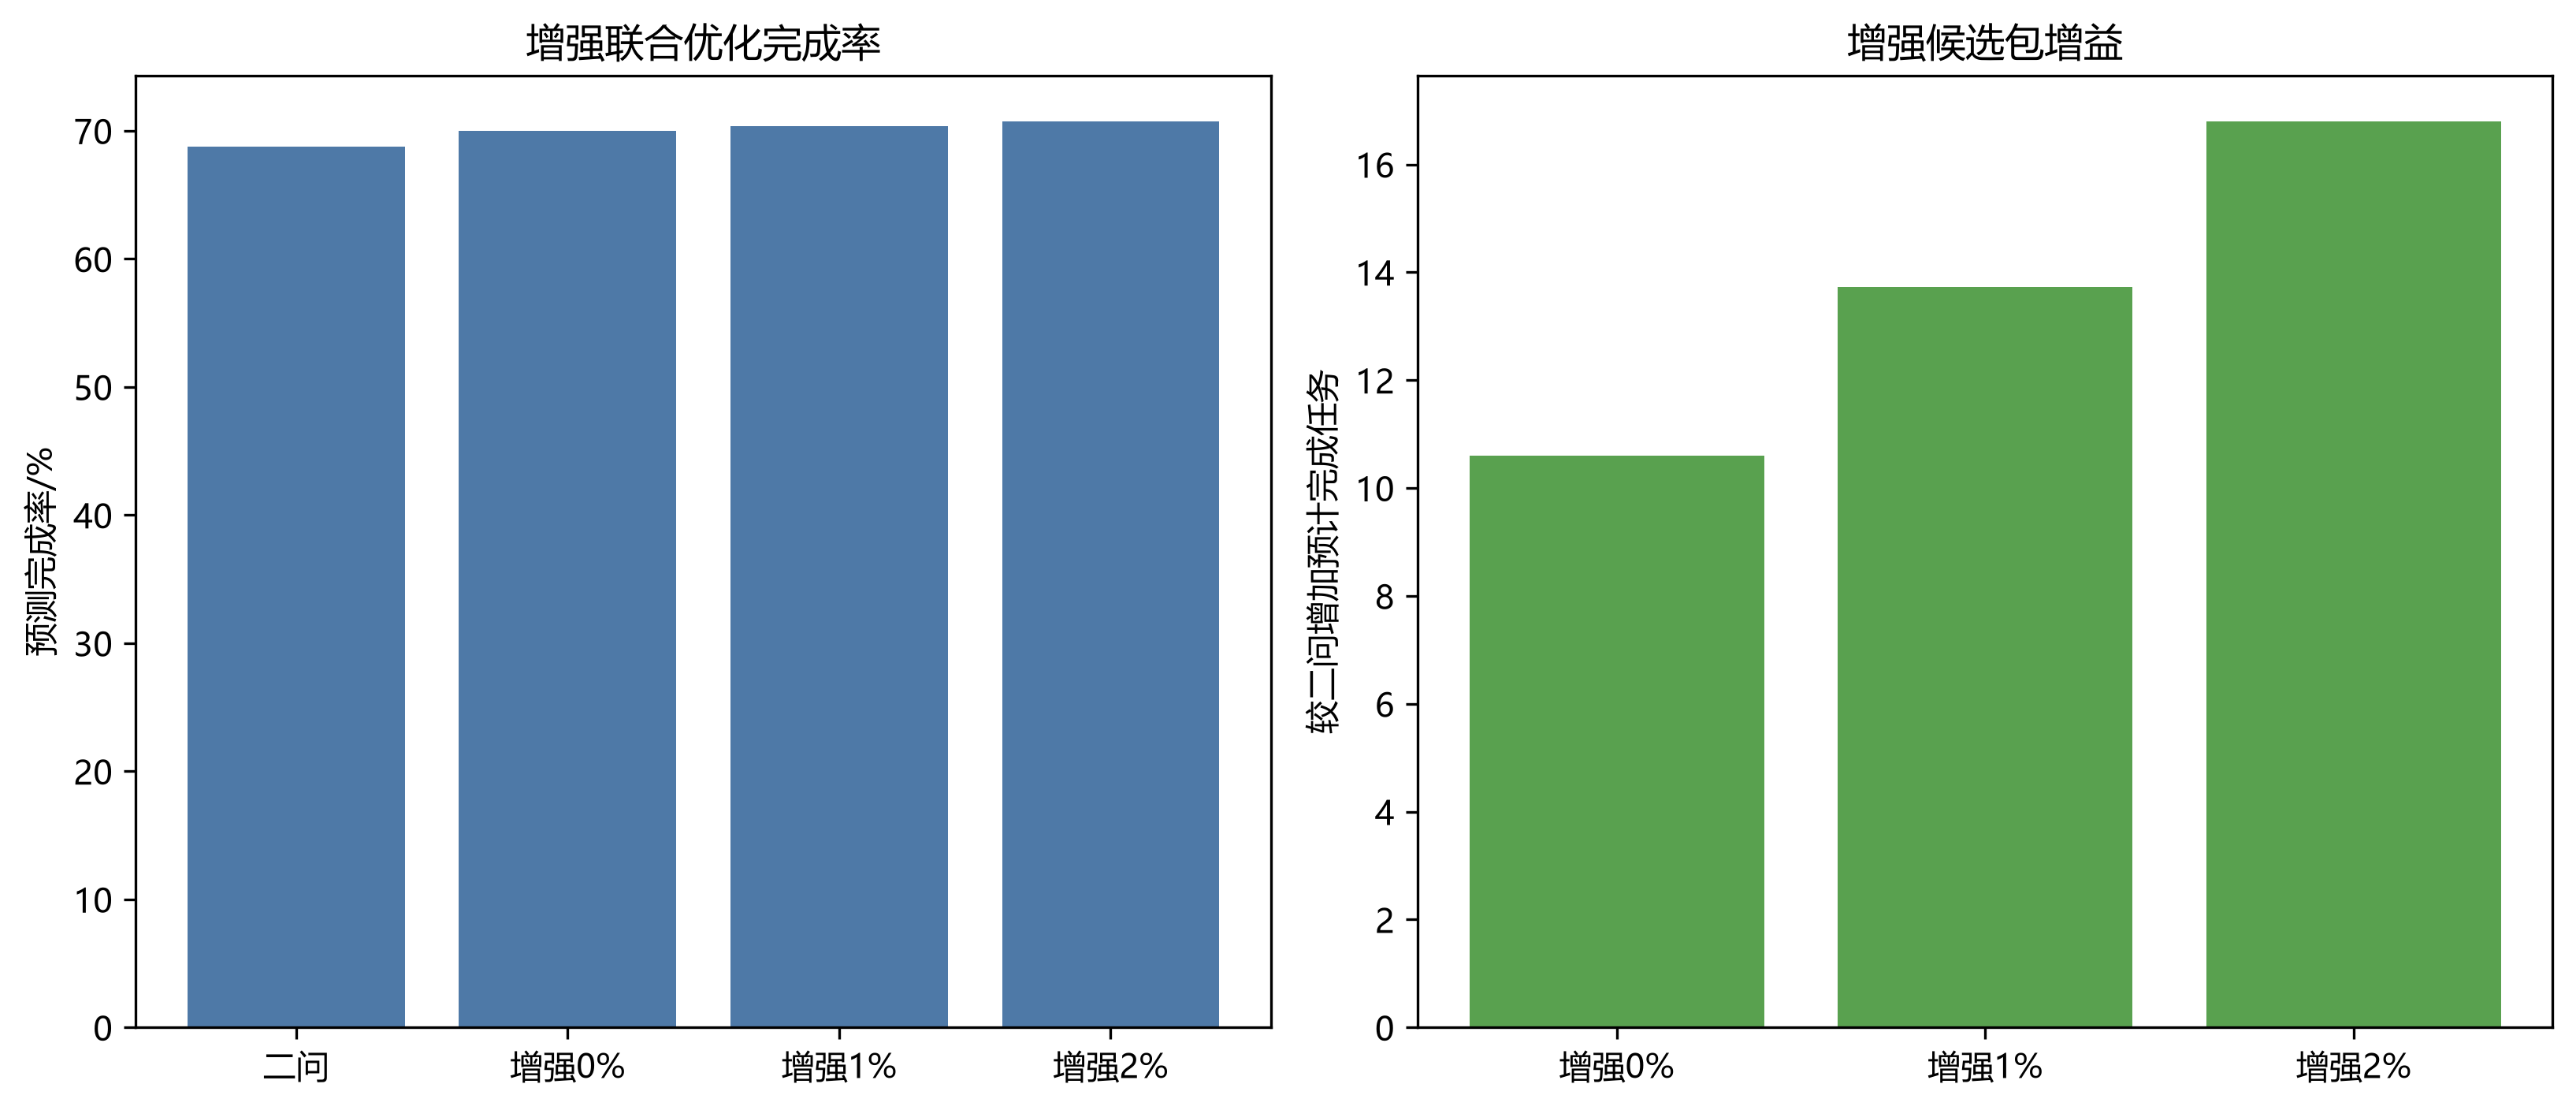
\includegraphics[width=0.78\textwidth]{../figures/question3-bundle-comparison.png}
\caption{问题三不同预算下联合打包定价的预测结果}
\label{fig:q3-bundle}
\end{figure}

同预算方案选择46个任务包，覆盖120个任务，其中11个为顺路搭配任务，其余715个任务单独发布。预计完成率由68.74\%提高到70.01\%，说明提升并非来自追加预算，而来自发布结构和预算配置的共同改变。包内路线共享提高低概率任务的相对吸引力，覆盖约束又允许未入包任务重新选择单价，因而不存在“打包收益”与“单价优化收益”重复计算的问题。

预算增加1\%和2\%时预计完成数继续增加，但每增加约419元预算所换取的新增完成数从首个情景的结构性收益转为约3个，体现边际收益下降。故若平台重视成本效率，应先实施同预算方案；若更重视覆盖率，可在热点区域试行1\%预算方案。由于包概率参数不是历史拟合量，70.01\%应解释为模型情景值。最需要观测的是任务包曝光、领取、部分完成、取消和真实路线，用于检验“整包领取即整包完成”的假设。

\subsection{约束核验与参数讨论}

联合解首先通过任务覆盖核验：120个入包任务和715个单独发布任务恰好构成全部835项任务，任一任务都没有同时出现在两个任务包或同时选择单任务价格。其次，预计支付41910.79元比问题二预算41910.85元少0.06元，说明完成数增加不是由求解器越过预算造成。第三，三个预算情景的MILP均返回最优状态，数值间隙约为$10^{-6}$；因此在给定候选包和式\eqref{eq:bundle-prob}参数的条件下，表\ref{tab:q3-results}反映的是离散方案的全局最优选择，而非贪心顺序的偶然结果。

参数风险主要来自包级概率，而不是整数规划本身。规模收益系数过大时，模型会偏好较大任务包；路线惩罚过大时，又会退化为单任务发布。本文通过把包规模限制为2--5项、距离限制为1 km，并比较三个预算情景，控制参数外推范围。实际试验可采用分层随机发布：在相似密度和问题二概率的任务中，一组按单任务发布，另一组使用2项或3项包，比较领取率、整包完成率、部分完成率和单位完成任务支付。只有当真实整包完成概率稳定高于包内单任务概率基准时，才扩大包规模。

任务包还可能造成选择权减少。若某个包包含一项显著偏远任务，较高总酬金也未必补偿完整路线成本；若包内任务时间窗口冲突，则几何紧凑并不等于可执行。因此上线前应增加最大道路时间、共同时间窗和包内最低单项概率三类筛选条件。现有附件没有道路和时间窗数据，本文没有虚构这些约束的数值效果，而把它们作为部署阶段的可核验条件。

从作用对象看，问题二主要修复所有任务的价格配置，问题三则只针对调价后仍困难的空间簇。二者的增量分别为51.96个和10.60个预计完成任务，量级差异符合递进逻辑：价格调整解决普遍性错配，打包解决剩余路线协同问题。若把两项提升简单相加而不联合求解，会忽略入包任务原单价被替换及预算重新分配，产生重复计算；式\eqref{eq:cover}正是防止该偏差的关键。

因此，打包方案的有效性同时表现为预算守恒、覆盖完整和预计完成数增加，而不能只用任务包数量判断。

\subsection{问题三结论}

在不增加问题二预计支付金额时，联合模型选择46个任务包、覆盖120项任务，使预测完成数增加10.60个并达到584.55个，预测完成率为70.01\%。任务打包主要改善已达到调价边界的密集低概率任务，是单任务定价的补充而非替代；推荐先采用同预算方案小规模发布，再依据真实包级数据校准式\eqref{eq:bundle-prob}。

\section{问题四：新任务的容量约束定价}

\subsection{新旧任务分布差异}

附件三包含2066个新任务，但没有标价和完成状态，故不能直接用历史平均价填充。把新任务代入历史空间特征后，新任务的任务--会员压力显著高于历史范围：按有效会员供给修正后的历史压力95\%分位数为3.248，而新任务中位数达到12.178。若把超出历史支持范围的密度直接输入Logistic模型，会产生不可靠的外推。因此对模型输入按历史95\%分位截尾，并另设拥挤修正项；这样既保留历史模型的相对规律，也明确承认新批次比历史批次更集中。

对会员$j$定义可执行权重$w_j$，综合信誉、预订限额和到任务的距离衰减；任务$i$的有效供给为
\begin{equation}
 S_i^{\rm eff}=\sum_j w_j\exp(-\lambda d_{ij})I(d_{ij}\leq r_s),
 \qquad R_i=\frac{1+G_i}{1+S_i^{\rm eff}}.
 \label{eq:effective-supply}
\end{equation}
$R_i$刻画附近任务对可执行会员容量的压力。与只数注册会员相比，这一指标避免把远距离、低限额会员等同于即时供给。历史任务用于估计价格响应，新任务只参与特征计算、候选包生成和优化，不把模型预测当作新观测。

\subsection{候选发布单元与会员容量}

新任务密集程度不同，固定包大小容易在中心区形成过长路线、在稀疏区又错失协同。本文按局部压力自适应生成2--4项的紧凑包，限制包内路线和最大距离，并保留单任务作为候选发布单元。对每个发布单元$g$和可服务会员$j$设指派变量$u_{gj}$；会员预订限额$q_j$形成
\begin{equation}
 \sum_g |S_g|u_{gj}\leq q_j,\qquad
 \sum_j u_{gj}=z_g.
 \label{eq:member-capacity}
\end{equation}
式\eqref{eq:member-capacity}要求被选择的发布单元恰好指派给一名满足距离条件的会员，并保证其承担任务数不超过限额。价格候选仍位于65--85元，目标是在原打包方案预计支付117106.43元以内最大化预计完成数，同时对过大包、过长路线和供给紧张区域施加惩罚。先求解包选择MILP，再求解会员指派MILP；两阶段分别控制发布结构和容量可行性，最终对未能指派的候选回退为单任务。

\subsection{方案结果与可行性}

\begin{table}[H]
\centering
\caption{附件三新任务定价方案的模型预测比较}
\begin{tabular}{lrrrr}
\toprule
方案 & 平均价/元 & 预计支付/元 & 预计完成数 & 完成率/\%\\
\midrule
统一75元单任务 & 75.00 & 77627.67 & 1035.04 & 50.10\\
逐任务定价 & 84.29 & 107485.51 & 1277.47 & 61.83\\
原打包模型 & 81.73 & 117106.43 & 1437.67 & 69.59\\
原方案按有效供给重估 & 81.73 & 102119.76 & 1253.34 & 60.67\\
容量约束优化打包 & 84.11 & 111842.52 & 1332.11 & 64.48\\
\bottomrule
\end{tabular}
\label{tab:q4-results}
\end{table}

\begin{figure}[H]
\centering
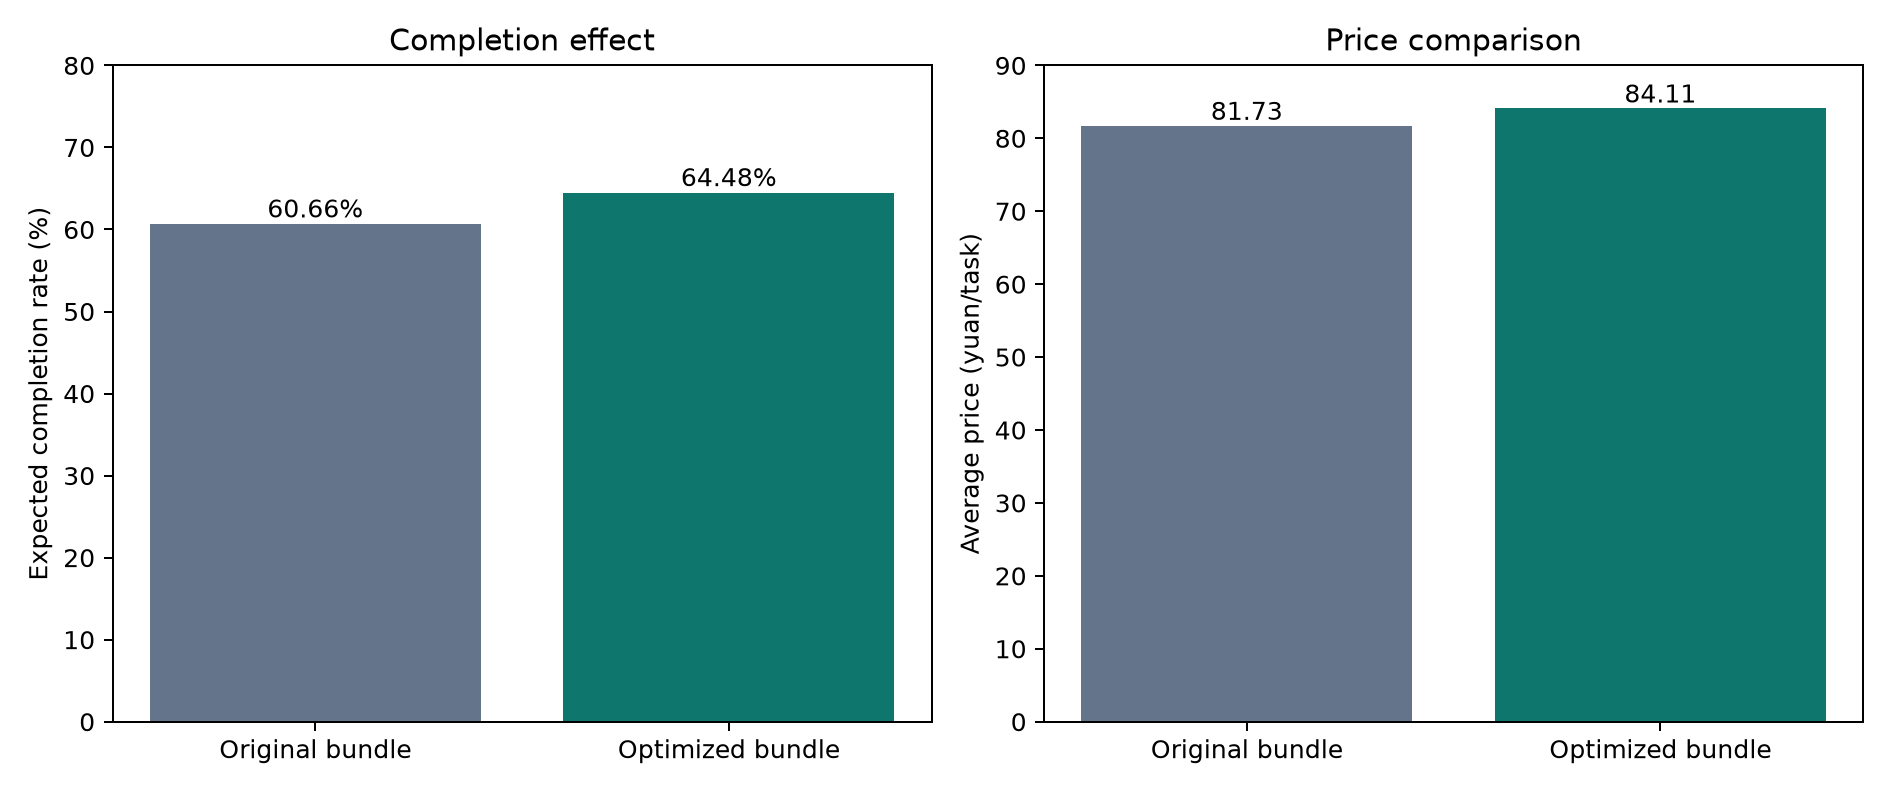
\includegraphics[width=0.78\textwidth]{../figures/question4-scheme-comparison.png}
\caption{问题四容量约束优化与原打包方案比较}
\label{fig:q4-scheme}
\end{figure}

原打包模型的69.59\%没有充分考虑有效供给不足。用新压力指标重估后，同一价格方案仅得到60.67\%，说明直接报告原值会高估密集新任务的可完成性。容量约束优化方案在同一预算上限内把完成率提高到64.48\%，比重估基线增加78.78个预计完成任务和3.81个百分点，因此将其作为问题四推荐方案。

推荐方案形成971个发布单元，其中709个多任务包覆盖1804项任务；共分配391名会员，最大容量利用率为1.000，无会员超过预订限额，最大包规模为4。平均单价84.11元，标价总额173776元，预计支付111842.52元，低于预算上限。1704项任务达到85元，且1680项即使在85元下仍不能达到0.75目标概率，说明问题四的主要矛盾已不再是小幅调价，而是新任务集中程度超过现有有效会员容量。此时继续加价既受价格上限限制，也不能替代新增供给。

\subsection{迁移校准与稳健性检查}

问题四最重要的检查是分布迁移。历史压力95\%分位数为3.248，而新任务压力中位数为12.178，后者约为前者的3.75倍。若不截尾，Logistic线性预测量会在训练数据没有覆盖的范围内继续变化，得到形式上精确但不可验证的概率。本文将历史特征截断在支持边界，并把超出部分转为显式拥挤惩罚，因而优化结果只利用历史模型能够辨识的排序信息。原打包价格按有效供给重估后完成率从69.59\%降至60.67\%，这一9个百分点差异直接说明迁移修正是必要步骤。

容量约束提供第二层可行性检查。优化后391名会员承担所选发布单元，会员最大利用率等于1但超限人数为0，说明预订限额约束满足；包选择求解器间隙为0，指派模型间隙为0.00443，在问题规模下能够支持实施比较。最大包规模为4，避免把大量集中任务交给单一会员。仍需注意，预订限额只表示平台允许的任务数量，不等于会员在特定时段真实在线，因此“无超限”是必要条件而不是完成保证。

为评估价格上限的作用，可观察达到85元的1704项任务和仍无法达到目标概率的1680项任务。两者高度重合表明大多数困难任务已经触及可选价格边界，若单纯放宽预算，优化仍会把资金集中到这些任务，却不一定获得相同比例的完成数增加。更稳健的措施是把任务按空间网格和时段分批释放，并在供给不足网格临时提高招募强度。试运行时应逐日比较预测概率与实际完成率，利用可靠性曲线重新校准截距；若某网格连续高估，则提高该网格的压力惩罚，而不是在全市统一修正。

三种基础方案还揭示了价格与组织方式的不同作用。统一75元方案平均价最低，但没有按空间压力区分任务，预测完成率只有50.10\%；逐任务定价把平均价提高到84.29元后达到61.83\%，说明差异化价格有效；容量约束打包在平均价略低的84.11元下达到64.48\%，表明路线协同和容量匹配提供了额外收益。该比较使用同一预测口径，因而可以评价相对方案，但不能替代真实上线后的因果试验。

从城市和网格层面还应分别统计预测完成率、实际完成率、平均等待时间和单位完成支付。若总体指标改善但个别网格持续恶化，应增加网格服务下限或减少跨网格打包；若会员容量普遍满载，则应把招募和分时释放置于进一步加价之前。该监测规则把问题一识别的区域异质性延续到新任务实施阶段，也使问题四方案能够随真实供给变化滚动修正。

实施时应分三层处理。第一层直接发布高概率单任务；第二层发布已指派会员、路线紧凑的任务包；第三层将达到85元仍低概率的任务延迟到供给较充足时段，或面向邻近区域招募会员。平台应先在若干空间网格试运行，记录实际领取和容量占用，再滚动更新$S_i^{\rm eff}$。如果实际完成率低于预测，应优先修正会员在线权重和包部分完成机制，而不是机械突破85元上限。

\subsection{问题四结论}

对2066个新任务，推荐容量约束优化打包方案：平均价格84.11元，选择971个发布单元，其中709个多任务包覆盖1804项任务；指派391名会员且无超限。模型预测完成1332.11项、完成率64.48\%，预计支付111842.52元。结果同时表明1680项任务在85元下仍难达到0.75目标概率，因此应把补充有效会员供给和分时发布作为价格方案的配套措施。\aimark{5}

\section{模型评价与改进}

\subsection{模型优点}

第一，模型把经纬度、会员能力与任务密度连接成可核对的证据链，并用城市残差约束未观测机制表述，避免把拥堵等背景变量误写成因果结论。第二，四问共享同一历史完成概率口径，单任务定价、任务打包和新任务迁移形成连续决策链。第三，预计支付、调价幅度、任务唯一覆盖、区域服务与会员容量被显式写成约束，结果具有可执行检查项。

模型还兼顾了可解释性与可求解性：候选价格先转化为概率--成本矩阵，使非线性预测与整数优化分离；精确MILP与贪心基线的结果接近，最优性间隙约为$10^{-6}$，说明当前离散方案的求解误差很小。区域服务下限、边界任务数及会员容量均能逐项核验，便于平台定位约束冲突并复查推荐价格，而不是只获得一个无法解释的总体目标值。

四问之间还保持了统一而递进的决策口径。问题一识别低价、有效供给不足、区域差异和任务竞争，问题二将这些因素转化为逐任务完成概率并重新分配预算；问题三只对调价后仍困难的空间簇引入路线协同，避免把打包收益与单价收益重复计算；问题四则在同一概率口径上增加会员容量和任务唯一覆盖约束。由此，每一问的新增结构都能追溯到前一问尚未解决的限制，数值结果也能在预计完成数、预计支付和约束可行性三个层面交叉核对。

模型的实施输出也较完整。推荐方案不仅给出总体完成率，还保留逐任务价格、区域变化、任务包组成和会员指派结果；预算敏感性分析显示成本中性、不同预算增幅和不同调价边界下的连续变化。因此平台可以先采用较保守的情景试行，再根据实际目标在成本、覆盖率和价格稳定性之间选择，而无需重新设计整个求解框架。

\subsection{模型局限与可执行改进}

完成概率模型采用线性预测子和统一价格系数，难以表达价格与空间环境的高阶交互、阈值及区域异质性；区域虚拟变量还会把区内差异压缩为平均效应。模型又将任务视为条件独立，局部竞争只作为静态特征进入，一项任务调价不会同步改变其他任务的选择概率，可能高估密集区域同时提价的收益。可用广义加性模型或单调树模型刻画非线性，并建立会员--任务匹配或离散选择模型处理任务替代。

优化模型默认各任务价值相同，且加权和只能给出固定偏好下的单个折中解；惩罚系数、价格网格及区域阈值都会影响方案，应补充Pareto前沿和联合敏感性分析。任务包概率还忽略部分完成与包内相关性，新任务模型依赖历史区域校准，分布变化时可能失准。后续应以试运行数据估计包级联合概率，并用迁移学习或分层贝叶斯方法更新参数。

\begin{thebibliography}{99}
  \bibitem{macqueen1967}
  MacQueen J. Some methods for classification and analysis of multivariate observations[C]//Proceedings of the Fifth Berkeley Symposium on Mathematical Statistics and Probability. Berkeley: University of California Press, 1967, 1: 281--297.

  \bibitem{hosmer2013}
  Hosmer D W, Lemeshow S, Sturdivant R X. Applied Logistic Regression[M]. 3rd ed. Hoboken: Wiley, 2013. DOI: \url{10.1002/9781118548387}.

  \bibitem{dantzig1957}
  Dantzig G B. Discrete-variable extremum problems[J]. Operations Research, 1957, 5(2): 266--288. DOI: \url{10.1287/opre.5.2.266}.

  \bibitem{openai2026}
  OpenAI. Codex[CP/OL]. 2026-07-24. \url{https://openai.com/codex/}.
\end{thebibliography}

\CumcmMainMatterEnd
\appendix
\ctexset{section={name={附录,、},number=\Alph{section}}}

\section{关键结果与支撑材料清单}

表\ref{tab:support-files}给出支撑四问主要结论、方案选择与约束核验的关键CSV结果，以及AI使用详情文件。清单不收录临时测试和重复中间结果，赛题原始附件不重复放入压缩包。

\begin{longtable}{L{0.29\textwidth}L{0.12\textwidth}L{0.39\textwidth}}
  \caption{四个问题的关键结果与支撑材料文件清单}
  \label{tab:support-files}\\
  \toprule
  文件名 & 对应问题 & 用途及输入输出 \\
  \midrule
  \endfirsthead
  \toprule
  文件名 & 对应问题 & 用途及输入输出 \\
  \midrule
  \endhead
  \supportfile{../support/data/question1-logistic-effects.csv}{question1-logistic-effects.csv}{问题一}{调整优势比、Bootstrap区间和模型指标}
  \supportfile{../support/data/question1-price-group-stats.csv}{question1-price-group-stats.csv}{问题一}{不同价格区间的任务数量与完成率}
  \supportfile{../support/data/question1-quantitative-model-metrics.csv}{question1-quantitative-model-metrics.csv}{问题一}{多因素模型拟合与分类指标}
  \supportfile{../support/data/question2-pricing-results.csv}{question2-pricing-results.csv}{问题二}{835个任务的原价、推荐价格和预测概率}
  \supportfile{../support/data/question2-milp-comparison.csv}{question2-milp-comparison.csv}{问题二}{贪心、精确MILP与实用MILP总体比较}
  \supportfile{../support/data/question2-milp-regional-comparison.csv}{question2-milp-regional-comparison.csv}{问题二}{各区域价格转移与完成率变化}
  \supportfile{../support/data/question2-completion-scenarios.csv}{question2-completion-scenarios.csv}{问题二}{不同预算与调价上限的敏感性结果}
  \supportfile{../support/data/question3-bundle-comparison.csv}{question3-bundle-comparison.csv}{问题三}{三种预算情景与问题二基线对比}
  \supportfile{../support/data/question3-joint-selected-options.csv}{question3-joint-selected-options.csv}{问题三}{联合模型最终选中的单任务与任务包方案}
  \supportfile{../support/data/question3-regional-summary.csv}{question3-regional-summary.csv}{问题三}{打包方案的区域分布与结果汇总}
  \supportfile{../support/data/question4-scheme-comparison.csv}{question4-scheme-comparison.csv}{问题四}{容量约束方案与原打包方案对比}
  \supportfile{../support/data/question4-bundle-packages.csv}{question4-bundle-packages.csv}{问题四}{新任务最终任务包组成与包价格}
  \supportfile{../support/data/question4-member-capacity.csv}{question4-member-capacity.csv}{问题四}{会员指派数量、限额与容量占用}
  \supportfile{../support/data/question4-city-summary.csv}{question4-city-summary.csv}{问题四}{新任务方案的城市级结果汇总}
  \supportfile{../support/AI 工具使用详情.pdf}{AI 工具使用详情.pdf}{全文}{记录AI辅助写作、排版、采纳内容与人工核验范围}
  \bottomrule
\end{longtable}

\section{可运行代码文件清单}

表\ref{tab:code-files}按问题列出关键代码文件。每问内部按数据准备、模型分析、优化求解或结果检验等主要环节细分，但不再拆分到单个函数。

\begin{longtable}{L{0.34\textwidth}L{0.12\textwidth}L{0.34\textwidth}}
  \caption{四个问题的关键代码文件清单}
  \label{tab:code-files}\\
  \toprule
  文件名 & 对应问题 & 关键环节 \\
  \midrule
  \endfirsthead
  \toprule
  文件名 & 对应问题 & 关键环节 \\
  \midrule
  \endhead
  \supportfile{../support/code/question1-complete.py}{question1-complete.py}{问题一}{数据清洗、描述统计与基础结果汇总}
  \supportfile{../support/code/question1-city-quantitative.py}{question1-city-quantitative.py}{问题一}{城市划分、区域供需指标与城市差异分析}
  \supportfile{../support/code/question1-quantitative-causes.py}{question1-quantitative-causes.py}{问题一}{多因素Logistic模型、Bootstrap区间与效应估计}
  \supportfile{../support/code/question1-external-quantitative.py}{question1-external-quantitative.py}{问题一}{外部空间变量构造与扩展稳健性分析}
  \supportfile{../support/code/question2-complete.py}{question2-complete.py}{问题二}{定价流程入口与主要结果整合}
  \supportfile{../support/code/question2-baseline-pricing.py}{question2-baseline-pricing.py}{问题二}{候选价格生成、完成概率估计与基准方案}
  \supportfile{../support/code/question2-milp-pricing.py}{question2-milp-pricing.py}{问题二}{预算约束下的精确与实用MILP定价}
  \supportfile{../support/code/question2-scenario-analysis.py}{question2-scenario-analysis.py}{问题二}{预算、价格上限与完成率敏感性分析}
  \supportfile{../support/code/question3-complete.py}{question3-complete.py}{问题三}{任务打包流程入口与结果汇总}
  \supportfile{../support/code/question3-bundle-simulation.py}{question3-bundle-simulation.py}{问题三}{候选任务包生成与包完成概率模拟}
  \supportfile{../support/code/question3-joint-bundle-milp.py}{question3-joint-bundle-milp.py}{问题三}{单任务与任务包联合选择模型}
  \supportfile{../support/code/question3-enhanced-joint-bundle-milp.py}{question3-enhanced-joint-bundle-milp.py}{问题三}{紧凑候选包筛选与增强联合优化}
  \supportfile{../support/code/question4-complete.py}{question4-complete.py}{问题四}{新任务数据处理、基础打包与方案评价}
  \supportfile{../support/code/question4-optimized.py}{question4-optimized.py}{问题四}{自适应任务包、会员容量约束与最终优化}
  \bottomrule
\end{longtable}

\end{document}
